\documentclass[11pt,a4paper]{article}

\usepackage[utf8]{inputenc}
\usepackage[T1]{fontenc}
\usepackage{amsmath,amssymb,amsthm}
\usepackage{mathtools}
\usepackage{booktabs}
\usepackage{graphicx}
\usepackage{tikz}
\usetikzlibrary{arrows.meta,positioning}
\usepackage[margin=1in]{geometry}
\usepackage{natbib}
\usepackage{enumitem}
\usepackage{hyperref}
\usepackage{cleveref}
\emergencystretch=2em

\theoremstyle{plain}
\newtheorem{theorem}{Theorem}
\newtheorem{lemma}[theorem]{Lemma}
\newtheorem{proposition}[theorem]{Proposition}
\newtheorem{corollary}[theorem]{Corollary}
\theoremstyle{definition}
\newtheorem{definition}[theorem]{Definition}
\newtheorem{example}[theorem]{Example}
\theoremstyle{remark}
\newtheorem{remark}[theorem]{Remark}

\newcommand{\E}{\mathbb{E}}
\newcommand{\Prob}{\mathbb{P}}
\newcommand{\R}{\mathbb{R}}
\newcommand{\KL}{\mathrm{KL}}
\newcommand{\cmin}{c^{\min}}
\newcommand{\astar}{a^\star}
\newcommand{\Env}{\mathcal{E}}

\title{Who pays for exploration?\\[2pt]
\large Per-person regret when a collective learns a public policy}
\author{Alexander Telfar}
\date{Draft, November 2026}

\begin{document}
\maketitle

\begin{abstract}
When a planner learns which policy is best by trying policies, the cost of learning is usually summarised by a single number, the regret. If the policy is a public good, applying to everyone at once, each person bears a different share of that cost, and regret is a vector with one entry per person. We study this vector in a stochastic bandit with public arms and Gaussian rewards. For a planner that targets total welfare we show that (i) observing every person's reward does not lower the Lai--Robbins rate at which worse policies must be tried, though it is needed to know who is paying; (ii) every asymptotically optimal planner imposes the same per-person burden, which falls on people who lose from policies that are nearly optimal in total; (iii) over all consistent planners the achievable burdens form a translated convex cone; and (iv) the people whose burden no consistent planner can reduce are exactly those for whom the welfare-optimal policy is also their favourite. Minimising the largest burden is a linear program, and in most random instances it cannot improve on the utilitarian planner at all. We then drop the requirement that the planner settle on one policy. Holding several policies in rotation is a far stronger lever, and near-ties, which are the most costly to resolve by exploring, are the cheapest to share. With a status quo as baseline, we define a person's privilege as how close the status quo is to their favourite policy, show that a planner unwilling to impose any expected loss on anyone can never try anything, and give a planner that keeps every person within a stated tolerance of the status quo in every round, by construction, with regret of order $T^{2/3}$. We compare this with compensation: paying each person their status-quo reward and sharing the surplus turns the per-person floors into one pooled floor on welfare, equalises the burden of learning at its lower bound, and lowers a bound on the trials needed before a reform can be adopted, at the price of assuming that rewards are transferable and honestly observed. A finite-horizon example shows that a welfare-maximising planner tries reforms it expects to be worse than the status quo, and that switching costs and fixed terms mainly change which reforms are tried.
\end{abstract}

% ======================================================================
\section{Introduction}\label{sec:intro}
% ======================================================================

A planner who does not know which policy is best has to try some. In the standard account of this problem, the multi-armed bandit, the cost of trying is regret: the reward forgone, relative to always using the best policy, while the planner finds out which one that is. The theory is mostly about keeping regret small, and its central result is that it cannot be made very small: any planner that eventually settles on the best policy must try each worse policy a number of times that grows logarithmically with the horizon, at a rate fixed by how hard that policy is to distinguish from the best \citep{lai1985}.

That account assumes the agent that explores is the agent that pays. Many collective decisions do not have this form. A tax rule, a curriculum, a safety standard, or the behaviour of a deployed AI system applies to everyone affected at the same time. When such a policy is tried and turns out worse, the loss is not spread evenly; some people lose a great deal, and some people gain, because they preferred the policy that was being tested. The planner's regret is the sum of these individual losses, but the sum hides who paid.

This paper asks a narrow question about that hidden distribution. If a planner learns in the standard way, aiming at total welfare, who carries the cost of the learning, and how much can the planner do about it?

\paragraph{Public arms.} The feature that makes the question non-trivial is that the arms are \emph{public}: a single policy is chosen each round and applies to the whole population. This is what separates legislation from a clinical trial. In a trial, the experimental treatment can be assigned to some patients and not others, so the experimenter can choose who is exposed; trials randomise exposure, cap it with stopping rules, and require consent \citep{freedman1987}. \citet{baek2021,baek2024} study fair exploration in a setting of this kind, where each round belongs to one group, and show that the choice of \emph{who} explores is a powerful lever. With public arms that lever does not exist (\cref{fig:setup}). For a planner that must settle on the welfare-best policy, the only remaining lever is how often each other policy is tried. A planner that may hold several policies in rotation has a second lever, which we take up in \cref{sec:sharing}.

\begin{figure}[t]\centering
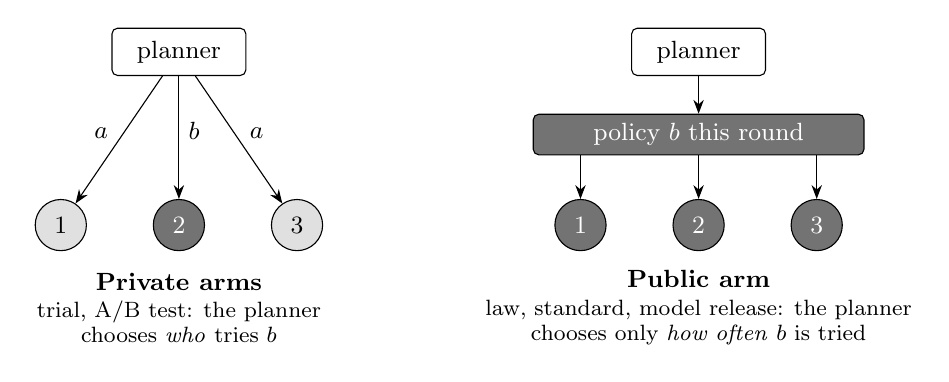
\begin{tikzpicture}[
  font=\small, >={Stealth[length=5pt]},
  planner/.style={draw, rounded corners=2pt, minimum width=17mm, minimum height=6mm},
  person/.style={circle, draw, minimum size=6.5mm, inner sep=0pt},
  A/.style={fill=black!12}, B/.style={fill=black!55, text=white}]
  % private arms
  \begin{scope}
    \node[planner] (p) at (0,2.2) {planner};
    \node[person,A] (x1) at (-1.5,0) {1};
    \node[person,B] (x2) at (0,0) {2};
    \node[person,A] (x3) at (1.5,0) {3};
    \draw[->] (p) -- node[left=2pt,pos=.45] {$a$} (x1);
    \draw[->] (p) -- node[right=0pt,pos=.45] {$b$} (x2);
    \draw[->] (p) -- node[right=2pt,pos=.45] {$a$} (x3);
    \node[align=center] at (0,-1.05) {\textbf{Private arms}\\[-1pt]\footnotesize trial, A/B test: the planner\\[-2pt]\footnotesize chooses \emph{who} tries $b$};
  \end{scope}
  % public arm
  \begin{scope}[xshift=6.6cm]
    \node[planner] (p) at (0,2.2) {planner};
    \node[draw, rounded corners=2pt, B, minimum width=42mm, minimum height=5mm] (pol) at (0,1.15) {policy $b$ this round};
    \node[person,B] (y1) at (-1.5,0) {1};
    \node[person,B] (y2) at (0,0) {2};
    \node[person,B] (y3) at (1.5,0) {3};
    \draw[->] (p) -- (pol);
    \foreach \y in {y1,y2,y3} \draw[->] (pol.south -| \y) -- (\y);
    \node[align=center] at (0,-1.05) {\textbf{Public arm}\\[-1pt]\footnotesize law, standard, model release: the planner\\[-2pt]\footnotesize chooses only \emph{how often} $b$ is tried};
  \end{scope}
\end{tikzpicture}
\caption{Private and public arms. With private arms the planner can decide who is exposed to an experimental policy. With a public arm everyone is exposed at once, and each person's cost is fixed by how much they lose under that policy.}
\label{fig:setup}
\end{figure}

\paragraph{Motivation from AI deployment.} The setting describes several practices in the governance of AI systems. A model update shipped to all users of a product is a public arm for that product's users. A staged rollout, a limited release or a regulatory sandbox is an attempt to turn a public arm into a partly private one, by choosing a population that bears the early risk. Our results quantify what is at stake in that choice: when it is not available, the burden of learning falls on a population determined by the instance, and the planner's freedom to redistribute it is small.

\paragraph{Three sources of loss.} Measured against their own favourite policy, a person loses in three ways. They lose because the collective settles on a policy that is best in total and not best for them (\emph{conflict}); because the institution may settle on something other than the best in total, for instance when it sees only votes (\emph{distortion}); and because nobody knew at the start which policy was best (\emph{learning}). The first two grow linearly with the horizon and the third logarithmically. Most of this paper is about the third, which is the part due to ignorance and the part a learning algorithm controls. It is the smallest of the three at long horizons, and we say so here because the per-person learning cost should not be read as the whole of what a person gives up. \Cref{sec:sharing,sec:sq} bring the first term back in; the second we leave to future work (\cref{sec:limits}).

\paragraph{Contributions.} We consider $N$ people, $K$ policies and jointly Gaussian rewards with known covariance. Person $i$'s regret is $R_i(T)=\sum_t(\mu_{i,\astar}-\mu_{i,a_t})$, where $\astar$ is the welfare-best policy, so that utilitarian regret is $\sum_iR_i$.
\begin{enumerate}[leftmargin=*,itemsep=2pt]
  \item \textbf{Individual observations do not help find $\astar$} (\cref{thm:lower}). Even a planner who sees every person's reward must try each suboptimal policy $a$ at least $(2\sigma^2/\Delta_a^2)\log T$ times, where $\Delta_a$ is the welfare gap and $\sigma^2$ is the variance of total reward. This is the Lai--Robbins rate for a planner who sees only the total. Individual observations are still needed to know who is paying.
  \item \textbf{The per-person burden of an asymptotically optimal planner} (\cref{thm:exact}) is $b_i=2\sigma^2\sum_{a}\delta_{i,a}/\Delta_a^2$ per unit of $\log T$, where $\delta_{i,a}$ is person $i$'s loss from policy $a$ relative to $\astar$. It is largest for people who lose from policies that are nearly optimal in total, and it can exceed the whole collective's regret, because others gain.
  \item \textbf{The achievable set is a cone} (\cref{thm:cone}). Over all consistent planners, the limit points of $\E[R(T)]/\log T$ are exactly $\{Dc: c\ge\cmin\}$, where $D$ is the matrix of individual gaps. A person's burden is irreducible exactly when $\astar$ is their favourite policy (\cref{cor:irreducible}); per-person budgets are feasible if and only if a linear system is (\cref{cor:budget}).
  \item \textbf{Min-max burden} (\cref{prop:lp,prop:ville}). Minimising the largest burden over the cone is a linear program. The utilitarian planner cannot be improved on exactly when some weighted average of the worst-off people weakly prefers $\astar$ to every alternative, which holds in roughly 80--93\% of random instances.
  \item \textbf{Time-sharing} (\cref{sec:sharing}). A planner that holds several policies in rotation moves per-person outcomes on the scale of $T$. The smallest largest conflict loss is a linear program with the same alternative condition, applied to different people, and the opposite conclusion: time-sharing helps in 90--100\% of random instances.
  \item \textbf{Status quo, privilege and individual rationality} (\cref{sec:sq}). With a status quo as baseline we define privilege (\cref{def:privilege}), show that a planner that tolerates no expected loss for anyone can never try anything (\cref{prop:nofree}), characterise when unanimity blocks all reform (\cref{prop:weights}), and give a planner that keeps every person within a tolerance of the status quo in every round (\cref{prop:safe}), with regret of order $T^{2/3}$ against the best time-share that respects the tolerance (\cref{prop:regret}).
  \item \textbf{Guarantees or compensation} (\cref{sec:comp}). Paying each person their status-quo reward and sharing the surplus gives everyone the same multiple of the collective's gain, attains the lower bound on the largest burden (\cref{prop:insure}), and replaces $N$ floors by one. We bound from below the trials needed before a reform can be held under each kind of floor; the pooled bound is never larger (\cref{prop:certify}).
  \item \textbf{A scorecard of institutions} (\cref{sec:score}). On one example we score institutions with and without transfers on welfare and each person's gain over the status quo, at horizons from $30$ to $30{,}000$ rounds.
  \item \textbf{Short horizons and frictions} (\cref{sec:finite}). In a one-reform problem solved numerically, the welfare-maximising planner tries reforms it expects to be worse than the status quo, and switching costs and fixed terms raise the bar for trying.
\end{enumerate}

Items 1 and 2 are routine consequences of known lower bounds once the problem is posed. The public-arm model itself is that of \citet{hossain2021}; the programme of describing the achievable per-group costs of exploration and choosing a fair point in it is due to \citet{baek2021}. What is new here, as far as we know, is the per-person account on a public arm: the cone and its irreducible part, the two alternative conditions, and the status-quo analysis.

% ======================================================================
\section{Setting}\label{sec:setting}
% ======================================================================

There are $N$ people and $K$ policies (arms). An \emph{instance} $\nu$ is a matrix of means $\mu\in\R^{N\times K}$; the noise covariance $\Sigma\in\R^{N\times N}$ is positive definite, known and fixed. In each round $t=1,\dots,T$ the planner chooses an arm $a_t$ and observes the reward vector
\[
  X_t=\mu_{\cdot,a_t}+\xi_t,\qquad \xi_t\sim\mathcal N(0,\Sigma)\ \text{ i.i.d.}
\]
Two cases to keep in mind are independent noise, $\Sigma=\mathrm{diag}(\sigma_1^2,\dots,\sigma_N^2)$, and independent noise plus a shock of variance $\tau^2$ common to everyone, $\Sigma=\mathrm{diag}(\sigma_i^2)+\tau^2\mathbf 1\mathbf 1^\top$. The planner's choice of $a_t$ may depend on $X_1,\dots,X_{t-1}$, on $a_1,\dots,a_{t-1}$, and on independent internal randomness. A planner that observes less (for example only $\sum_iX_{t,i}$) is a special case.

The welfare of arm $a$ is $W(a)=\sum_i\mu_{i,a}$. We let $\Env$ denote the class of all instances $\mu\in\R^{N\times K}$ with a unique welfare maximiser $\astar=\astar(\nu)$. This class is \emph{unstructured}: knowing the means of one arm says nothing about another. Write
\[
  \delta_{i,a}=\mu_{i,\astar}-\mu_{i,a},\qquad \Delta_a=W(\astar)-W(a)=\sum_i\delta_{i,a},\qquad \sigma^2=\mathbf 1^\top\Sigma\mathbf 1 .
\]
Here $\sigma^2$ is the variance of the total reward $\sum_iX_{t,i}$; it is $\sum_i\sigma_i^2$ with independent noise and $\sum_i\sigma_i^2+N^2\tau^2$ with a common shock. For $a\neq\astar$, $\Delta_a>0$, while $\delta_{i,a}$ may have either sign. Let $n_a(T)$ be the number of rounds up to $T$ in which arm $a$ was chosen.

\begin{definition}[Per-person regret]
Person $i$'s regret is $R_i(T)=\sum_{t=1}^T(\mu_{i,\astar}-\mu_{i,a_t})=\sum_{a\neq\astar}n_a(T)\,\delta_{i,a}$, and the regret vector is $R(T)=(R_1(T),\dots,R_N(T))$. Utilitarian regret is $\sum_iR_i(T)=\sum_{a}n_a(T)\Delta_a$.
\end{definition}

Two features of this definition matter. First, $R_i$ is measured against $\astar$, not against person $i$'s favourite arm, so it isolates the cost of learning from the cost of living under a utilitarian choice. Second, $R_i$ can be negative: a person who prefers an arm that is being tested does better while it is tested. Write $m_i=\max_a\mu_{i,a}$ for the reward of person $i$'s favourite policy and $\rho_i=m_i-\mu_{i,\astar}\ge0$ for their \emph{conflict loss} under $\astar$. Against their own favourite, person $i$ loses
\begin{equation}\label{eq:decomp}
  \sum_{t=1}^T(m_i-\mu_{i,a_t})=T\rho_i+R_i(T),
\end{equation}
a conflict term that is linear in $T$ and a learning term that, for the planners of \cref{sec:exact,sec:cone}, is logarithmic. In \cref{ex:blog} below, persons 1 and 2 have $\rho_i=0.5$ and person 3 has $\rho_3=0$.

Since $R_i$ is linear in the counts,
\begin{equation}\label{eq:linear}
  \E[R(T)]=D\,\E[n(T)],\qquad D=(\delta_{i,a})_{i\le N,\;a\neq\astar}\in\R^{N\times(K-1)},
\end{equation}
where $n(T)=(n_a(T))_{a\neq\astar}$. Everything below is a statement about $\E[n(T)]$, pushed through $D$.

\begin{definition}[Consistency and asymptotic optimality]\label{def:consistent}
A planner is \emph{consistent} on $\Env$ if for every $\nu\in\Env$, every $a\neq\astar(\nu)$ and every $p>0$, $\E_\nu[n_a(T)]=o(T^p)$. It is \emph{asymptotically optimal} if it is consistent and, for every $\nu\in\Env$,
\[
  \limsup_{T\to\infty}\frac{\sum_{a\neq\astar}\Delta_a\E_\nu[n_a(T)]}{\log T}\le\sum_{a\neq\astar}\Delta_a\,\cmin_a,\qquad \cmin_a:=\frac{2\sigma^2}{\Delta_a^2}.
\]
\end{definition}

Consistency is the usual minimal requirement: a planner that is not consistent has polynomial regret on some instance, which here means some population is subjected to a worse policy for a polynomial fraction of the time.

% ======================================================================
\section{Individual observations do not lower the exploration rate}\label{sec:lower}
% ======================================================================

\begin{lemma}[Cheapest way to make an arm look optimal]\label{lem:kl}
Let $m\in\R^N$, let $\Sigma$ be positive definite and let $\Delta>0$. Then
\[
  \min\Big\{\KL\big(\mathcal N(m,\Sigma)\,\|\,\mathcal N(m+d,\Sigma)\big):\ d\in\R^N,\ \mathbf 1^\top d=\Delta\Big\}=\frac{\Delta^2}{2\sigma^2},\qquad \sigma^2=\mathbf 1^\top\Sigma\mathbf 1,
\]
attained uniquely at $d^\star=\Delta\,\Sigma\mathbf 1/\sigma^2$.
\end{lemma}

\begin{proof}
For Gaussians with a common covariance, $\KL(\mathcal N(m,\Sigma)\|\mathcal N(m+d,\Sigma))=\tfrac12d^\top\Sigma^{-1}d$. By the Cauchy--Schwarz inequality,
\[
  \Delta^2=\big((\Sigma^{1/2}\mathbf 1)^\top(\Sigma^{-1/2}d)\big)^2\le\big(\mathbf 1^\top\Sigma\mathbf 1\big)\big(d^\top\Sigma^{-1}d\big),
\]
so $\tfrac12d^\top\Sigma^{-1}d\ge\Delta^2/(2\sigma^2)$, with equality if and only if $\Sigma^{-1/2}d$ is proportional to $\Sigma^{1/2}\mathbf 1$, that is $d=\lambda\Sigma\mathbf 1$; the constraint gives $\lambda=\Delta/\sigma^2$. With independent noise, $d^\star_i=\Delta\sigma_i^2/\sigma^2$.
\end{proof}

\begin{theorem}[Lower bound with vector observations]\label{thm:lower}
Let the planner be consistent on $\Env$. For every $\nu\in\Env$ and every $a\neq\astar(\nu)$,
\[
  \liminf_{T\to\infty}\frac{\E_\nu[n_a(T)]}{\log T}\ \ge\ \cmin_a=\frac{2\sigma^2}{\Delta_a^2}.
\]
\end{theorem}

\begin{proof}
Fix $\nu$, $a\neq\astar$ and $\varepsilon>0$. Let $d\in\R^N$ with $\sum_id_i=\Delta_a+\varepsilon$, and let $\nu'$ be the instance that agrees with $\nu$ except that column $a$ of the mean matrix is $\mu_{\cdot,a}+d$. Then $W'(a)=W(\astar)+\varepsilon$ and $W'(b)=W(b)$ for $b\neq a$, so $a$ is the unique optimal arm of $\nu'$ and $\nu'\in\Env$.

Let $\Prob_\nu$, $\Prob_{\nu'}$ be the laws of the planner's full history (internal randomness, actions and observed vectors) up to time $T$ under the two instances. The two instances differ only in the distribution of the observation produced by arm $a$, so the divergence decomposition (\citealp[Lemma~15.1]{lattimore2020}, which holds for observations in any measurable space, in particular $\R^N$) gives
\[
  \KL(\Prob_\nu\|\Prob_{\nu'})=\E_\nu[n_a(T)]\cdot\KL\big(\mathcal N(\mu_{\cdot,a},\Sigma)\,\|\,\mathcal N(\mu_{\cdot,a}+d,\Sigma)\big)=:\E_\nu[n_a(T)]\,\kappa(d).
\]
Let $A=\{n_a(T)>T/2\}$. By the Bretagnolle--Huber inequality \citep[Theorem~14.2]{lattimore2020},
\[
  \Prob_\nu(A)+\Prob_{\nu'}(A^c)\ \ge\ \tfrac12\exp\big(-\KL(\Prob_\nu\|\Prob_{\nu'})\big).
\]
By Markov's inequality, $\Prob_\nu(A)\le 2\E_\nu[n_a(T)]/T$. On $A^c$, $\sum_{b\neq a}n_b(T)\ge T/2$, so $\Prob_{\nu'}(A^c)\le 2\sum_{b\neq a}\E_{\nu'}[n_b(T)]/T$. Hence
\[
  S_T:=\E_\nu[n_a(T)]+\sum_{b\neq a}\E_{\nu'}[n_b(T)]\ \ge\ \frac T4\exp\big(-\E_\nu[n_a(T)]\,\kappa(d)\big).
\]
Arm $a$ is suboptimal under $\nu$ and every $b\neq a$ is suboptimal under $\nu'$, so by consistency, for every $p>0$ we have $S_T\le T^p$ for all sufficiently large $T$. Taking logarithms,
\[
  \E_\nu[n_a(T)]\,\kappa(d)\ \ge\ \log\frac T4-\log S_T\ \ge\ (1-p)\log T-\log 4
\]
for all large $T$, so $\liminf_T\E_\nu[n_a(T)]/\log T\ge(1-p)/\kappa(d)$. Since $p>0$ was arbitrary, the bound holds with $1$ in place of $1-p$. Choosing $d$ as in \cref{lem:kl} with $\Delta=\Delta_a+\varepsilon$ gives $\kappa(d)=(\Delta_a+\varepsilon)^2/(2\sigma^2)$, and letting $\varepsilon\downarrow0$ gives the claim.
\end{proof}

\begin{remark}[Why individual observations do not help]\label{rem:noinfo}
The right-hand side is the Lai--Robbins constant for a scalar Gaussian bandit with variance $\sigma^2$, which is what a planner observing only the welfare signal $Y_t=\sum_iX_{t,i}\sim\mathcal N(W(a_t),\sigma^2)$ faces. \Cref{prop:upper} shows that such a planner attains it. So in the unstructured class $\Env$, seeing each person's reward gives no asymptotic advantage in finding $\astar$. The reason is \cref{lem:kl}: the cheapest confusing perturbation spreads the welfare shift across people in the direction $\Sigma\mathbf 1$, and its cost depends only on the size of the shift and on $\sigma^2$, the variance of the total. In a structured class, where the means of different arms are linked (for example by a low-dimensional preference model), individual observations can carry information about other arms and the constant changes; the general form is given by \citet{graves1997} (see also \citealp{combes2017}). We do not treat that case.

The remark has a second half. The welfare signal identifies $\astar$ but not the matrix $D$ of individual gaps: two instances with the same column sums are indistinguishable to a planner that sees only the total. So individual observations are not needed to learn efficiently, and they are needed to know who is paying for the learning. Every planner in \cref{sec:fair,sec:sharing,sec:sq} that aims at a fairer outcome uses them.
\end{remark}

% ======================================================================
\section{The burden imposed by an asymptotically optimal planner}\label{sec:exact}
% ======================================================================

\begin{proposition}[Achievability using only the total]\label{prop:upper}
Let a planner observe only $Y_t=\sum_iX_{t,i}$ and run the asymptotically optimal UCB algorithm of \citet[Chapter~8]{lattimore2020} on $Y_t/\sigma$, with index $\hat W_a/\sigma+\sqrt{2\log f(t)/n_a(t-1)}$ and $f(t)=1+t\log^2t$. Then the planner is consistent on $\Env$ and, for every $\nu\in\Env$ and $a\neq\astar$, $\limsup_T\E_\nu[n_a(T)]/\log T\le\cmin_a$. In particular it is asymptotically optimal.
\end{proposition}

\begin{proof}
$Y_t/\sigma$ is a unit-variance Gaussian bandit with gaps $\Delta_a/\sigma$. \citet[Theorem~8.1]{lattimore2020} gives, for every $\epsilon\in(0,\Delta_a/\sigma)$, a bound of the form $\E[n_a(T)]\le 1+5\epsilon^{-2}+2(\Delta_a/\sigma-\epsilon)^{-2}\big(\log f(T)+\sqrt{\pi\log f(T)}+1\big)$. % CHECK: constants as stated in the cited theorem
This is $O(\log T)$ on every instance, which gives consistency, and dividing by $\log T$ and letting $T\to\infty$ and then $\epsilon\to0$ gives the limsup bound since $\log f(T)/\log T\to1$.
\end{proof}

Thompson sampling with a flat prior on the welfare signal is also asymptotically optimal for Gaussian rewards with known variance \citep{korda2013}; KL-UCB is another option \citep{cappe2013}.

\begin{theorem}[Exact per-person burden]\label{thm:exact}
For every asymptotically optimal planner, every $\nu\in\Env$ and every $a\neq\astar$, $\E_\nu[n_a(T)]/\log T\to\cmin_a$. Consequently, for every person $i$,
\[
  \lim_{T\to\infty}\frac{\E_\nu[R_i(T)]}{\log T}=b_i:=\sum_{a\neq\astar}\delta_{i,a}\,\cmin_a=2\sigma^2\sum_{a\neq\astar}\frac{\delta_{i,a}}{\Delta_a^2}.
\]
\end{theorem}

\begin{proof}
Write $x_a(T)=\E_\nu[n_a(T)]/\log T$. By \cref{thm:lower}, $\liminf_Tx_b(T)\ge\cmin_b$ for every $b\neq\astar$. Fix $a$. For any sequences, $\limsup(u+v)\ge\limsup u+\liminf v$, so
\begin{align*}
  \Delta_a\limsup_Tx_a(T)\ &\le\ \limsup_T\sum_{b}\Delta_bx_b(T)-\sum_{b\neq a}\Delta_b\liminf_Tx_b(T)\\
  &\le\ \sum_b\Delta_b\cmin_b-\sum_{b\neq a}\Delta_b\cmin_b=\Delta_a\cmin_a,
\end{align*}
using asymptotic optimality for the first sum. Hence $\limsup_Tx_a(T)\le\cmin_a\le\liminf_Tx_a(T)$ and the limit exists. The second claim follows from \eqref{eq:linear}.
\end{proof}

\paragraph{Shares.} Writing $\kappa_{i,a}=\delta_{i,a}/\Delta_a$ for person $i$'s share of arm $a$'s welfare gap ($\sum_i\kappa_{i,a}=1$), the burden is $b_i=2\sigma^2\sum_a\kappa_{i,a}/\Delta_a$: a sum, over policies, of the person's share times how hard the policy is to rule out. A policy that is nearly optimal in total and polarising has small $\Delta_a$ and shares far from $1/N$, some negative and some above $1$.

\paragraph{The burden follows the benefit.} The gap $\delta_{i,a}$ plays two roles. It is what person $i$ loses in each round that $a$ is tried, and it is what person $i$ gains in every later round from $a$ having been ruled out in favour of $\astar$. So the people who pay to rule out a policy are the people who benefit from its being ruled out, in proportion to how much they benefit. This is the benefit principle of public finance. It does not make the burden small, and it does not help a person who would have been content with either policy's rival, but it does mean that the burden is not arbitrary.

\paragraph{How much would have to move.} If the burdens could be evened out by transfers, the amount that would have to change hands is $\tfrac12\sum_i|b_i-\bar b|$ per unit of $\log T$, where $\bar b$ is the mean burden. This can be much larger than the collective's regret $\sum_ib_i$, because gains and losses cancel in the sum; it is still logarithmic in the horizon.

\paragraph{Population size and common shocks.} Replicate the population $k$ times with independent noise. Then $\Delta_a$ and $\sigma^2$ are both multiplied by $k$, so $\cmin_a$ and every $b_i$ are divided by $k$: a large population with purely idiosyncratic noise learns almost at once, and each person's burden is negligible. With a common shock, $\sigma^2=\sum_i\sigma_i^2+N^2\tau^2$ grows like $N^2$, and per-person burdens stay of order one however large the population. Policy outcomes are noisy mainly because of shocks that hit everyone, so the common-shock case is the relevant one, and it is why \cref{lem:kl} is stated for a general covariance.

\begin{example}[One polarising near-tie]\label{ex:blog}
Three people, three policies, independent noise with $\sigma_i=1$ (so $\sigma^2=3$):
\begin{center}\small
\begin{tabular}{lccccc}
\toprule
policy & person 1 & person 2 & person 3 & $W$ & $\Delta$\\
\midrule
$\astar$ & 1.0 & 1.0 & 1.0 & 3.0 & --\\
$b$ & 1.5 & 1.5 & $-0.1$ & 2.9 & 0.1\\
$c$ & 0.5 & 0.5 & 0.5 & 1.5 & 1.5\\
\bottomrule
\end{tabular}
\end{center}
Here $\cmin=(600,\,8/3)$ and $b=(-298.7,\,-298.7,\,661.3)$ in units of $\log T$, while utilitarian regret is $64\log T$. Person 3 pays about ten times the collective's total, almost all of it from ruling out $b$; persons 1 and 2 come out ahead (\cref{fig:example}). Evening out the burdens would take transfers of $640\log T$, ten times the collective's regret. Against \eqref{eq:decomp}, though, person 3 has no conflict loss, while persons 1 and 2 each give up $0.5$ per round for as long as $\astar$ is in force.
\end{example}

\begin{figure}[t]\centering
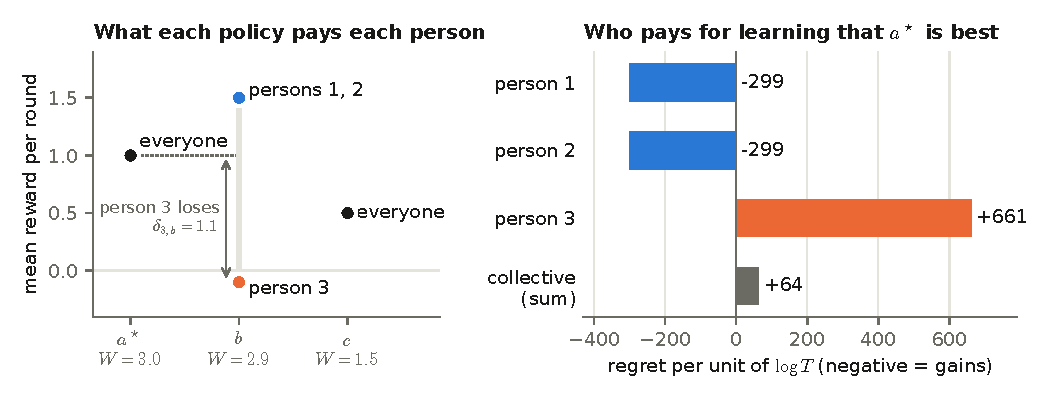
\includegraphics[width=\linewidth]{figures/fig_example.pdf}
\caption{\Cref{ex:blog}. Left: policy $b$ is almost as good as $\astar$ in total, but it moves $1.1$ per round from person 3 to persons 1 and 2. Right: the per-person burden of an asymptotically optimal planner (\cref{thm:exact}). The collective's regret is the small grey bar; it is the sum of one large loss and two large gains.}
\label{fig:example}
\end{figure}

% ======================================================================
\section{What any consistent planner can achieve}\label{sec:cone}
% ======================================================================

An asymptotically optimal planner has no freedom: \cref{thm:exact} fixes its burden vector. A merely consistent planner may try some policies more often than necessary, at a cost in total regret. The next theorem describes exactly which burden vectors this buys.

\begin{definition}
For $\nu\in\Env$, let $\mathcal L(\nu)\subseteq\R^N$ be the set of all finite limit points, as $T\to\infty$, of $\E_\nu[R(T)]/\log T$, taken over all planners that are consistent on $\Env$. Let
\[
  \mathcal C(\nu)=\{Dc:\ c\in\R^{K-1},\ c\ge\cmin\}
\]
(componentwise), a translate of the convex cone generated by the columns of $D$.
\end{definition}

\begin{theorem}[The achievable cone]\label{thm:cone}
For every $\nu\in\Env$, $\mathcal L(\nu)=\mathcal C(\nu)$. Moreover, for every $c\ge\cmin$ there is a planner, consistent on $\Env$, with $\E_\nu[n(T)]/\log T\to c$ and hence $\E_\nu[R(T)]/\log T\to Dc$.
\end{theorem}

The planner in the second statement depends on $\nu$ through the target $c$, but it is consistent on every instance. Whether a single planner can reach a chosen point of the cone (such as the min-max point of \cref{sec:fair}) on every instance simultaneously, without knowing $\nu$, is a different question, which we leave open (\cref{sec:limits}).

\begin{proof}[Proof of $\mathcal L(\nu)\subseteq\mathcal C(\nu)$]
Fix a consistent planner and let $x(T)=\E_\nu[n(T)]/\log T\in\R^{K-1}_{\ge0}$, so $\E_\nu[R(T)]/\log T=Dx(T)$. Suppose $Dx(T_k)\to r\in\R^N$ along some $T_k\to\infty$. Since $\mathbf 1^\top D=(\Delta_a)_{a\neq\astar}$ has strictly positive entries, $\min_a\Delta_a\cdot\|x(T_k)\|_1\le\mathbf 1^\top Dx(T_k)\to\mathbf 1^\top r$, so $(x(T_k))$ is bounded and has a further subsequence converging to some $c$. By \cref{thm:lower}, $c_a\ge\liminf_Tx_a(T)\ge\cmin_a$ for every $a$, and by continuity $r=Dc\in\mathcal C(\nu)$.
\end{proof}

The reverse inclusion uses a planner that adds a deterministic schedule of forced pulls to an asymptotically optimal base planner.

\begin{definition}[Forced exploration]\label{def:forced}
Let $g\in\R^K_{\ge0}$ and let $\pi_0$ be any planner. The planner $\pi_g$ keeps forced counts $f_b(t)$, initially $0$. In round $t$, if some arm $b$ has $f_b(t-1)<g_b\log t$, it pulls the arm with the largest deficit $g_b\log t-f_b(t-1)$ and increments its forced count; otherwise it performs one step of $\pi_0$, which sees only the outcomes of its own steps.
\end{definition}

Whether round $t$ is forced, and which arm it forces, depends only on $g$ and $t$, not on any observation. So the forced counts $f_b(T)$ and the number $S(T)$ of rounds handed to $\pi_0$ by time $T$ are deterministic, and the history of $\pi_0$'s own steps has the same law as a standalone run of $\pi_0$ for $S(T)$ rounds.

\begin{lemma}[The schedule keeps pace]\label{lem:schedule}
Let $G=\sum_bg_b$ and $M=G\log2+K$. For every $T$ with $T>2(G\log T+K)$ and every arm $b$,
\[
  g_b\log(T-M)\ \le\ f_b(T)\ \le\ g_b\log T+1,\qquad T-G\log T-K\ \le\ S(T)\ \le\ T.
\]
\end{lemma}

\begin{proof}
Upper bound: arm $b$ is forced in round $t$ only if $f_b(t-1)<g_b\log t\le g_b\log T$, after which $f_b(t)<g_b\log T+1$. Summing the upper bound over arms gives the lower bound on $S(T)$.

Lower bound: call round $t$ \emph{free} if $f_b(t-1)\ge g_b\log t$ for all $b$. If no round in $\{1,\dots,T\}$ is free, all $T$ rounds are forced, so $T\le\sum_b(g_b\log T+1)=G\log T+K$, which contradicts the hypothesis. So let $\tau\le T$ be the last free round. Every round in $\{\tau+1,\dots,T\}$ is forced, and in that interval arm $b$ is forced at most $g_b\log T+1-f_b(\tau)\le g_b\log(T/\tau)+1$ times, because $f_b(\tau)\ge f_b(\tau-1)\ge g_b\log\tau$. Hence $T-\tau\le G\log(T/\tau)+K$. If $\tau\le T/2$ this gives $T/2\le G\log T+K$, again contradicting the hypothesis; so $\tau>T/2$, and then $T-\tau\le G\log2+K=M$. Finally $f_b(T)\ge f_b(\tau-1)\ge g_b\log\tau\ge g_b\log(T-M)$.
\end{proof}

\begin{proof}[Proof of $\mathcal C(\nu)\subseteq\mathcal L(\nu)$ and of the second statement]
Let $c\ge\cmin$. Take $\pi_0$ asymptotically optimal (for example the planner of \cref{prop:upper}) and run $\pi_g$ with $g_a=c_a-\cmin_a$ for $a\neq\astar(\nu)$ and $g_{\astar(\nu)}=0$. Write $n^0_a(s)$ for the counts of a standalone run of $\pi_0$ after $s$ rounds. Then, on any instance $\nu''$,
\[
  \E_{\nu''}[n_a(T)]=f_a(T)+\E_{\nu''}[n^0_a(S(T))].
\]
\emph{Consistency.} By \cref{lem:schedule}, $f_a(T)=O(\log T)$; since $S(T)\le T$ and $\pi_0$ is consistent, $\E_{\nu''}[n^0_a(S(T))]=o(T^p)$ for every suboptimal $a$ of $\nu''$ and every $p>0$. So $\pi_g$ is consistent on $\Env$.

\emph{Limit on $\nu$.} By \cref{lem:schedule}, $f_a(T)/\log T\to g_a$. Also $S(T)\to\infty$ and $\log S(T)/\log T\to1$, so by \cref{thm:exact} applied to $\pi_0$,
\[
  \frac{\E_\nu[n^0_a(S(T))]}{\log T}=\frac{\E_\nu[n^0_a(S(T))]}{\log S(T)}\cdot\frac{\log S(T)}{\log T}\ \to\ \cmin_a .
\]
Hence $\E_\nu[n_a(T)]/\log T\to g_a+\cmin_a=c_a$ and $\E_\nu[R(T)]/\log T\to Dc$ by \eqref{eq:linear}.
\end{proof}

\subsection{Consequences}

\begin{corollary}[Irreducible burden]\label{cor:irreducible}
Let person $i$ weakly prefer $\astar$ to every arm, that is $\delta_{i,a}\ge0$ for all $a$. Then for every consistent planner
\[
  \liminf_{T\to\infty}\frac{\E_\nu[R_i(T)]}{\log T}\ \ge\ b_i=\sum_{a\neq\astar}\delta_{i,a}\cmin_a,
\]
with equality for every asymptotically optimal planner. If instead $\delta_{i,a}<0$ for some $a$, then $\inf\{r_i: r\in\mathcal C(\nu)\}=-\infty$: such a person's burden can be made arbitrarily negative on the $\log T$ scale, by trying an arm they prefer more often, at a utilitarian cost of $\Delta_a$ per unit.
\end{corollary}

\begin{proof}
With nonnegative coefficients, $\liminf_T\sum_a\delta_{i,a}x_a(T)\ge\sum_a\delta_{i,a}\liminf_Tx_a(T)\ge\sum_a\delta_{i,a}\cmin_a$ by \cref{thm:lower}. Equality is \cref{thm:exact}. The second statement follows from $c=\cmin+te_a$, $t\to\infty$, and \cref{thm:cone}.
\end{proof}

The condition $\delta_{i,a}\ge0$ for all $a$ says that $\astar$ is person $i$'s favourite policy, that is $\rho_i=0$ in \eqref{eq:decomp}. So the people whose learning burden cannot be reduced are exactly the people who have no conflict loss: the utilitarian optimum is the best policy there is for them, and the price is that they carry the cost of establishing it. Everyone else has a positive conflict loss and a learning burden that can be bought down.

If $b_i>0$, which holds whenever $\delta_{i,\cdot}\ge0$ and some $\delta_{i,a}>0$, person $i$'s expected regret grows without bound under every consistent planner. A fixed cap $\E[R_i(T)]\le B_i$, a right not to be experimented on beyond a fixed amount, cannot be honoured. The general version of the feasibility question is a linear program.

\begin{corollary}[Budgets]\label{cor:budget}
Let $\beta\in\R^N$. There is a consistent planner with $\limsup_T\E_\nu[R_i(T)]/\log T\le\beta_i$ for all $i$ if and only if there is $c\ge\cmin$ with $Dc\le\beta$.
\end{corollary}

\begin{proof}
If such $c$ exists, the planner of \cref{thm:cone} attains $Dc\le\beta$. Conversely, if a consistent planner satisfies the bounds then $\mathbf 1^\top Dx(T)=\sum_a\Delta_ax_a(T)$ is bounded above for large $T$, so $x(T)$ is bounded; a convergent subsequence has a limit $c\ge\cmin$ (\cref{thm:lower}) with $Dc\le\beta$.
\end{proof}

When the budgets are infeasible, something outside the model has to give: stop learning and accept regret linear in $T$, change the objective (which changes $\Delta$ and $D$), or remove arms from consideration in advance. The last option removes the burden of ruling out a contested arm, but if that arm is in fact optimal it costs a constant fraction of welfare forever.

% ======================================================================
\section{Min-max fairness}\label{sec:fair}
% ======================================================================

The cone makes the trade-off between the total cost of learning and its distribution explicit. A natural target is the smallest worst-off burden,
\[
  v^\star(\nu)=\min_{c\ge\cmin}\ \max_i\,(Dc)_i .
\]

\begin{proposition}\label{prop:lp}
$v^\star$ is the value of the linear program $\min\{t:\ Dc\le t\mathbf 1,\ c\ge\cmin\}$, which is attained. It satisfies
\[
  \max\Big\{\tfrac1N\textstyle\sum_a\Delta_a\cmin_a,\ \max_{i:\,\delta_{i,\cdot}\ge0}b_i\Big\}\ \le\ v^\star\ \le\ \max_ib_i .
\]
By \cref{thm:cone} it is the smallest worst-off burden achievable by a consistent planner, and the extra utilitarian regret it costs, the \emph{price of fairness}, is $\sum_a\Delta_a(c^\star_a-\cmin_a)$ per unit of $\log T$, where $c^\star$ is any optimal solution.
\end{proposition}

\begin{proof}
For any feasible $c$, $\max_i(Dc)_i\ge\frac1N\mathbf 1^\top Dc=\frac1N\sum_a\Delta_ac_a\ge\frac1N\sum_a\Delta_a\cmin_a$, so the LP is bounded below; a feasible linear program that is bounded below attains its optimum. For a person with $\delta_{i,\cdot}\ge0$, $(Dc)_i\ge(D\cmin)_i=b_i$ for all $c\ge\cmin$. The upper bound is $c=\cmin$.
\end{proof}

The next lemma is used three times, here and in \cref{sec:sharing,sec:sq}.

\begin{lemma}[An alternative]\label{lem:alt}
For any real matrix $M$, exactly one of the following holds: there is $e\ge0$ with $Me<0$ componentwise; or there is $y\ge0$, $y\neq0$, with $y^\top M\ge0$.
\end{lemma}

\begin{proof}
If $e\ge0$ has $Me<0$, then so does $e+\epsilon\mathbf 1$ for small $\epsilon>0$, so the first statement is equivalent to the solvability of $Me<0$, $-e<0$. By Gordan's theorem \citep[Ch.~2]{mangasarian1969}, this system is solvable if and only if there is no $(y,u)\ge0$, $(y,u)\neq0$, with $M^\top y-u=0$. Such a pair has $y^\top M=u^\top\ge0$ and $y\neq0$ (if $y=0$ then $u=0$); conversely any $y\ge0$, $y\neq0$, with $y^\top M\ge0$ gives the pair $(y,M^\top y)$.
\end{proof}

When does the utilitarian planner already achieve $v^\star$? Let $I=\{i:\ b_i=\max_jb_j\}$ be the people who are worst off under it, and $D_I$ the corresponding rows of $D$.

\begin{proposition}[When the largest burden cannot be reduced]\label{prop:ville}
$\cmin$ is optimal for the min-max problem if and only if there are weights $y\ge0$ on $I$, summing to one, with $y^\top D_I\ge0$; that is, if and only if some weighted average of the worst-off people weakly prefers $\astar$ to every alternative. In particular, if the worst-off person is unique, the largest burden can be reduced exactly when that person strictly prefers some policy to $\astar$.
\end{proposition}

\begin{proof}
$F(c)=\max_i(Dc)_i$ is convex and piecewise linear, and the feasible set is $\cmin+\R^{K-1}_{\ge0}$. Hence $\cmin$ is optimal if and only if the one-sided directional derivative $F'(\cmin;e)=\max_{i\in I}(De)_i$ is nonnegative for every $e\ge0$; the formula for $F'$ is the standard one for a maximum of finitely many linear functions, in which only the active ones matter. So $\cmin$ fails to be optimal if and only if there is $e\ge0$ with $D_Ie<0$ componentwise, and \cref{lem:alt} with $M=D_I$ gives the statement after normalising $y$.
\end{proof}

When the condition holds we say the utilitarian planner is \emph{unimprovable}. This is not a statement that its burdens are fair. In \cref{ex:blog} the condition holds and the burdens are $(-299,-299,661)$: the largest burden cannot be reduced because the person who carries it has no policy they prefer to $\astar$. Unimprovable means that redistribution through exploration is unavailable.

\begin{example}[Redistribution at a price]\label{ex:comp}
In \cref{ex:blog}, person 3 is the unique worst-off person and weakly prefers $\astar$ to both alternatives, so by \cref{prop:ville} no consistent planner can lower their burden of $661.3\log T$. Now add an arm $d$ with rewards $(0.6,0.6,1.6)$, so $W(d)=2.8$, $\Delta_d=0.2$, $\cmin_d=150$ and $\delta_{\cdot,d}=(0.4,0.4,-0.6)$. Under the utilitarian planner the burdens are $(-238.7,-238.7,571.3)$ and the total is $94\log T$. Person 3 now prefers $d$ to $\astar$, so trying $d$ more often helps them. The LP sets $c^\star_d=960$ (that is, $810$ extra pulls of $d$ per unit of $\log T$) and equalises all three burdens at $v^\star=256/3\approx85.3$. The price is $0.2\times810=162$ per unit of $\log T$, which nearly triples total regret, from $94$ to $256$. Redistribution through exploration is possible here only because the person who pays happens to like another policy that is cheap to try. \Cref{fig:cone} shows the cone for this example.
\end{example}

\begin{figure}[t]\centering
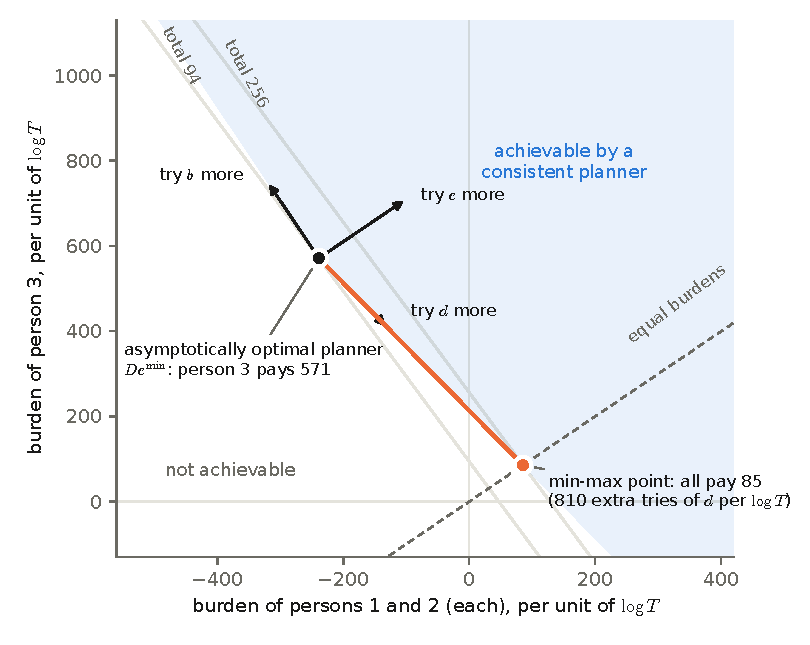
\includegraphics[width=0.72\linewidth]{figures/fig_cone.pdf}
\caption{The achievable set of \cref{thm:cone} for \cref{ex:comp}, projected on the burden of persons 1 and 2 (who are identical) and of person 3. The apex is the burden of every asymptotically optimal planner. Each arrow is the direction in which the burden moves when one arm is tried more often than necessary; the shaded cone is everything a consistent planner can reach. Grey lines join points with the same total regret. Moving from the apex to the min-max point uses only arm $d$, and raises total regret from $94$ to $256$ per unit of $\log T$.}
\label{fig:cone}
\end{figure}

% ======================================================================
\section{Time-sharing: the lever that consistency rules out}\label{sec:sharing}
% ======================================================================

\Cref{sec:cone,sec:fair} hold the target fixed: a consistent planner must end up at $\astar$, so it can only move burdens on the $\log T$ scale. A planner that is allowed to miss $\astar$ on purpose has a much stronger lever. It can hold several policies in rotation, each for a fixed fraction of the time. This is how the same public-arm model is treated by \citet{hossain2021} and \citet{jones2023}, who target the distribution over arms that maximises Nash welfare. This section asks what that lever does to the per-person accounts.

\begin{definition}[Time-share]
A \emph{time-share} is a distribution $p$ over the $K$ arms. Its long-run reward vector is $u(p)=\mu p$, its conflict loss for person $i$ is $\rho_i(p)=m_i-u_i(p)\ge0$, and its welfare price is $W(\astar)-\mathbf 1^\top\mu p=\sum_{a\neq\astar}p_a\Delta_a$ per round.
\end{definition}

Relative to $\astar$, a time-share that puts weight $q_a$ on each arm $a\neq\astar$ changes person $i$'s reward by $-(Dq)_i$ per round. These are the same generators as in \cref{thm:cone}: the columns of $D$, one per suboptimal arm. The cone of \cref{sec:cone} is what they generate on the $\log T$ scale, above the floor $\cmin$; time-sharing uses them on the scale of $T$, with no floor. Two things follow at once. Time-sharing can raise a person's reward only through an arm that person prefers to $\astar$. And the people it cannot help are those with $\delta_{i,\cdot}\ge0$, who by \cref{cor:irreducible} have no conflict loss to remove.

\paragraph{The smallest largest conflict loss.} The analogue of the min-max burden is
\[
  v_c(\nu)=\min_{p}\ \max_i\ \rho_i(p).
\]

\begin{proposition}\label{prop:share}
$v_c$ is the value of the linear program $\min\{t:\ m_i-(\mu p)_i\le t\ \forall i,\ p\ge0,\ \mathbf 1^\top p=1\}$, and it is attained by a time-share that uses at most $N+1$ arms. Let $J$ be the set of people with the largest conflict loss under $\astar$. The pure policy $\astar$ attains $v_c$ if and only if there are weights $y\ge0$ on $J$, summing to one, with $y^\top D_J\ge0$. In particular, if one person alone has the largest conflict loss and it is positive, some time-share does strictly better than $\astar$.
\end{proposition}

\begin{proof}
The program is the definition of $v_c$. The vector $u(p)$ lies in the convex hull of the $K$ columns of $\mu$ in $\R^N$, so by Carath\'eodory's theorem it is a mixture of at most $N+1$ of them. For the second claim, write a time-share as weight $q\ge0$ on the arms other than $\astar$, with $\mathbf 1^\top q\le1$. Then $\max_i\rho_i=\max_i[\rho_i(\astar)+(Dq)_i]$ is convex and piecewise linear in $q$, and the constraint $\mathbf 1^\top q\le1$ is inactive at $q=0$. So $q=0$ is optimal if and only if there is no direction $e\ge0$ with $D_Je<0$, and \cref{lem:alt} gives the condition. If $J=\{j\}$ and $\rho_j(\astar)>0$, person $j$ strictly prefers some arm to $\astar$, so row $j$ of $D$ has a negative entry and no $y$ exists.
\end{proof}

The condition has the same form as \cref{prop:ville}, with the people who have the largest conflict loss in place of the people who have the largest learning burden. Its consequences are opposite. The person with the largest learning burden usually prefers $\astar$ to everything, so nothing can be done for them. The person with the largest conflict loss never does, so something always can.

\begin{example}[Sharing a near-tie]\label{ex:share}
In \cref{ex:blog} the conflict losses under $\astar$ are $(0.5,0.5,0)$. Holding $b$ for a fraction $q_b$ of the time gives $(0.5-0.5q_b,\ 0.5-0.5q_b,\ 1.1q_b)$, which is equalised at $q_b=5/16$: every person then loses $0.344$ per round against their own favourite. The welfare price is $\Delta_bq_b=0.031$ per round, about $1\%$ of $W(\astar)$.
\end{example}

\paragraph{Near-ties are costly to resolve and cheap to share.} Ruling out arm $a$ costs the collective $\Delta_a\cmin_a=2\sigma^2/\Delta_a$ per unit of $\log T$, which is large when $\Delta_a$ is small. Sharing with arm $a$ costs $\Delta_a$ per unit of time, which is small when $\Delta_a$ is small. A polarising near-tie is therefore the case in which a utilitarian planner spends most of its exploration to settle a question whose answer matters least for total welfare and most for who gets it. In \cref{ex:blog}, telling $\astar$ from $b$ takes $600\log T$ rounds of $b$ and is worth $0.1$ per round in total; the same choice moves $1.1$ per round between people.

\paragraph{Random instances.} On the instance distribution of \cref{sec:numerics}, \cref{tab:share} reports how often some time-share has a smaller largest conflict loss than $\astar$, and by how much. Time-sharing helps in almost every instance, and it cuts the largest conflict loss by a third or more at the median. The same table recalls the corresponding numbers for the exploration lever of \cref{sec:fair}.

\begin{table}[h]\centering\small
\begin{tabular}{rrccc|c}
\toprule
& & \multicolumn{3}{c|}{time-sharing, largest conflict loss} & exploration, largest burden\\
$N$ & $K$ & can be reduced & median reduction & median price per person & can be reduced\\
\midrule
3 & 3 & 90\% & 34\% & 0.11 & 7\%\\
5 & 4 & 100\% & 40\% & 0.18 & 10\%\\
10 & 5 & 100\% & 41\% & 0.19 & 10\%\\
20 & 8 & 100\% & 42\% & 0.19 & 21\%\\
\bottomrule
\end{tabular}
\caption{400 random instances per row ($\mu_{i,a}\sim\mathcal N(0,1)$ i.i.d.). Medians are over instances in which a reduction is possible. The price is the welfare given up per person per round, in units of the standard deviation of $\mu_{i,a}$. The last column is one minus the second column of \cref{tab:freq}.}
\label{tab:share}
\end{table}

\paragraph{Learning a time-share.} We have described the target, not a planner that learns it. \citet{hossain2021} and \citet{jones2023} give planners with scalar regret of order $\sqrt T$ against the Nash-welfare time-share. Two observations bear on the per-person version, which we leave open. First, every arm in the support of the target is held for a constant fraction of the time, so it is sampled linearly often and there is no logarithmic exploration of it to pay for; only arms outside the support have to be ruled out. Second, the target depends on each person's means and not only on the totals, so a planner that learns it must observe individual rewards.

% ======================================================================
\section{The status quo, privilege, and individually rational exploration}\label{sec:sq}
% ======================================================================

So far every loss has been measured against $\astar$ or against a person's own favourite policy. People who object to a reform usually measure against something else: the policy already in force. This section adds a status quo and asks what can be learned without making anyone worse off than under it.

\subsection{The status quo as a baseline}

Let one arm, $a_0\neq\astar$, be the \emph{status quo}. It has been in force for a long time, so its means $\mu_{\cdot,a_0}$ are known. Person $i$'s gain from the planner's choices, relative to keeping the status quo, is
\[
  G_i(T)=\sum_{t=1}^T(\mu_{i,a_t}-\mu_{i,a_0})=T\,(\mu_{i,\astar}-\mu_{i,a_0})-R_i(T).
\]
The first term is person $i$'s stake in reform. It is linear in $T$ and it can be negative: the utilitarian optimum is a potential-compensation improvement on the status quo, in the sense of Kaldor and Hicks, and need not be a Pareto improvement.

\begin{definition}[Privilege]\label{def:privilege}
Person $i$'s \emph{status-quo regret} is $\rho^0_i=m_i-\mu_{i,a_0}$, the amount per round by which the status quo falls short of person $i$'s favourite policy. Person $i$ is \emph{more privileged} than person $j$ if $\rho^0_i<\rho^0_j$.
\end{definition}

Privilege in this sense is a fact about a person and a policy menu, not about the person alone. A person with $\rho^0_i=0$ has their favourite policy already. For them every trial of anything else is a loss, and no amount of redirected exploration can change that; this is \cref{cor:irreducible} with the baseline moved from $\astar$ to $a_0$. A person with large $\rho^0_i$ has the most to gain from some reform, though not necessarily from the one that is best in total.

Two remarks connect the definition to exploration.

\emph{Exploration is progressive in expectation.} Suppose that, before anything else has been tried, the planner regards the untried arms as exchangeable, and let $\bar m_i$ be the reward it expects person $i$ to get from any one of them. Trying an untried arm for one round then changes person $i$'s expected reward by $\bar m_i-\mu_{i,a_0}$. This is negative exactly for the people whom the status quo places above what they could expect from an arbitrary alternative, and it falls one for one as $\mu_{i,a_0}$ rises. So the people best served by the status quo expect to pay for experiments, and the people worst served expect to gain from them.

\emph{Not exploring is not neutral.} A planner that never leaves $a_0$ has $G_i(T)=0$ for everyone and imposes a loss of $T(\mu_{i,\astar}-\mu_{i,a_0})$ on everyone with a positive stake in reform. The status quo is an arm, and keeping it has a regret vector like any other choice \citep{meyer2015}.

\begin{example}[A status quo]\label{ex:sq}
Add to \cref{ex:blog} a status quo $a_0$ with rewards $(1.2,\,1.2,\,0.2)$, so $W(a_0)=2.6$. The status-quo regrets are $\rho^0=(0.3,\,0.3,\,0.8)$: persons 1 and 2 are the more privileged. Moving to $\astar$ raises welfare by $0.4$ per round, costs persons 1 and 2 $0.2$ each, and gives person 3 $0.8$. A planner that learns $\astar$ in the standard way must also rule out $a_0$ ($\Delta_{a_0}=0.4$, $\cmin_{a_0}=37.5$); its learning burdens are $(-306,\,-306,\,691)$ per unit of $\log T$ and total regret is $79\log T$.
\end{example}

\subsection{Individual rationality}

A constraint that protects each person relative to the status quo has to be stated per round, because a planner that is allowed to make a person worse off now on the promise of later gains is asking for exactly the trust that is in question.

\begin{definition}[Individually rational planner]\label{def:ir}
Let $p_t$ be the distribution from which the planner draws $a_t$, given the history. For $\alpha\ge0$ and $\delta\in(0,1)$, the planner is \emph{$\alpha$-individually rational with confidence $1-\delta$} on a class of instances if, on every instance in the class,
\[
  \Prob\big(\,(\mu p_t)_i\ \ge\ \mu_{i,a_0}-\alpha\ \text{ for all } i \text{ and all } t\,\big)\ \ge\ 1-\delta .
\]
\end{definition}

The tolerance $\alpha$ is the expected loss per round, relative to the status quo, that each person can be asked to accept. It may differ between people; we take it equal to keep the notation light. We work on the class $\Env_L$ of instances that share the known status-quo means and satisfy $|\mu_{i,a}-\mu_{i,a_0}|\le L$ for all $i$ and $a$, for a known $L>0$. Without some such bound a planner knows nothing at all about an untried arm.

\begin{proposition}[No free trial]\label{prop:nofree}
If a planner is $0$-individually rational with confidence $1-\delta$ on $\Env_L$, then on every instance in $\Env_L$ the probability that it ever plays an arm other than $a_0$ is at most $\delta$.
\end{proposition}

\begin{proof}
Let $\tau$ be the first round in which $p_\tau(a_0)<1$, with $\tau=\infty$ if there is none. Before $\tau$ only $a_0$ has been played, and the law of its observations is the same on every instance in $\Env_L$, so the probability of $\{\tau<\infty\}$ is the same on every instance. Let $\nu^-$ be the instance with $\mu_{i,a}=\mu_{i,a_0}-L$ for all $i$ and all $a\neq a_0$; it lies in $\Env_L$ and $a_0$ is its unique welfare maximiser. On $\nu^-$, if $\tau<\infty$ then $(\mu p_\tau)_i=\mu_{i,a_0}-L(1-p_\tau(a_0))<\mu_{i,a_0}$, which violates the constraint. So $\{\tau<\infty\}$ has probability at most $\delta$ on $\nu^-$, hence on every instance, and the planner cannot play another arm unless $\tau<\infty$.
\end{proof}

So a collective that will not accept any expected loss for anyone, even for one round, cannot learn anything. Experimenting on a public arm requires some tolerance, and $\alpha$ is where that requirement is made explicit.

\subsection{What an individually rational planner should aim at}

With the means known, the best a planner can do under the constraint is the time-share
\[
  p^\star_\alpha\in\arg\max_p\Big\{\mathbf 1^\top\mu p:\ \mu p\ge\mu_{\cdot,a_0}-\alpha\mathbf 1,\ p\ge0,\ \mathbf 1^\top p=1\Big\},
\]
a linear program, feasible because $p=e_{a_0}$ satisfies it. Its value $W_\alpha$ is concave and nondecreasing in $\alpha$. The optimal dual variable $\lambda_i$ on person $i$'s constraint is the welfare the collective would gain per round from one more unit of tolerance from person $i$. It is zero for anyone whose constraint is slack, and positive only for people whose protection is holding the collective back: it is the price of person $i$'s veto. In general the solution is a time-share and not a single policy, so individual rationality leads to \cref{sec:sharing} whether or not fairness was the aim.

\begin{proposition}[When unanimity blocks everything]\label{prop:weights}
The following are equivalent: (a) no time-share gives every person strictly more than the status quo; (b) there are welfare weights $w\ge0$, $w\neq0$, under which the status quo maximises $\sum_iw_i\mu_{i,a}$ over arms.
\end{proposition}

\begin{proof}
Let $A=\mu-\mu_{\cdot,a_0}\mathbf 1^\top\in\R^{N\times K}$. Statement (a) fails if and only if there is $p\ge0$ with $Ap>0$ (normalise $p$ to sum to one; $p=0$ is excluded by the strict inequality). By \cref{lem:alt} applied to $M=-A$, this is the alternative to the existence of $w\ge0$, $w\neq0$, with $w^\top A\le0$, which says $\sum_iw_i\mu_{i,a}\le\sum_iw_i\mu_{i,a_0}$ for every arm $a$.
\end{proof}

When such weights exist they are a second description of privilege: they say whose interests the status quo is optimal for. A status quo that no unanimous reform can improve is one that is exactly right for somebody's weighting of the population, and the further those weights are from equal, the more unequal the protection that unanimity gives.

\begin{example}\label{ex:ir}
In \cref{ex:sq} no weights rationalise $a_0$: they would need $w_3\ge w_1+w_2$ for $a_0$ to beat $b$ and $w_3\le(w_1+w_2)/4$ for it to beat $\astar$. So a unanimous improvement exists. The best one is $p^\star_0$: $\astar$ for $60\%$ of the time and $b$ for $40\%$, with rewards $(1.2,\,1.2,\,0.56)$ and welfare $2.96$ (\cref{fig:sharing}). Persons 1 and 2 are held exactly at their status-quo level and person 3 gains $0.36$. The collective gives up $0.04$ per round relative to $\astar$, and the price of the protection is $\lambda_1+\lambda_2=0.2$: each unit of tolerance from persons 1 and 2 together would buy $0.2$ of welfare. With $\alpha=0.05$ the target is $70\%$ $\astar$ and $30\%$ $b$, with welfare $2.97$.
\end{example}

\begin{figure}[t]\centering
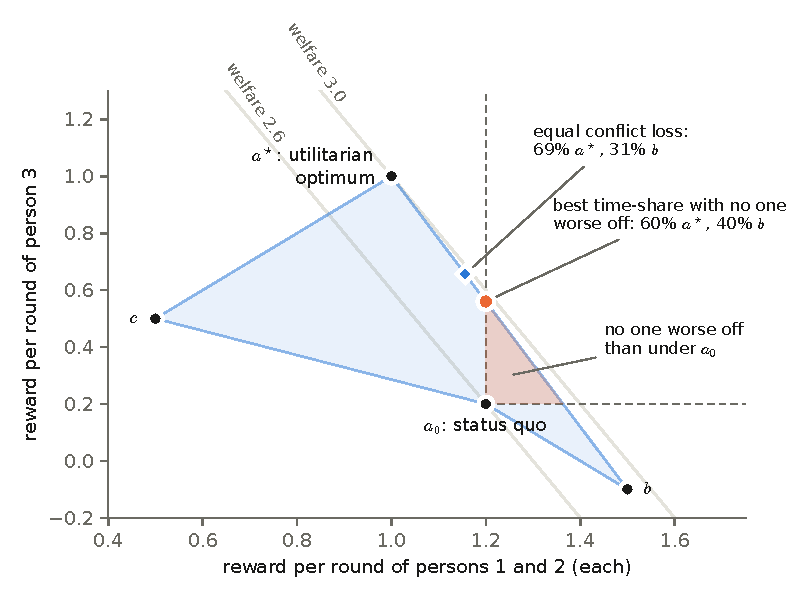
\includegraphics[width=0.72\linewidth]{figures/fig_sharing.pdf}
\caption{\Cref{ex:sq}: the reward vectors that time-sharing can reach (shaded blue), projected on persons 1 and 2 (identical) and person 3. The status quo $a_0$ lies inside the set, so some time-shares make everyone better off (shaded orange). The best of these in total is $60\%$ $\astar$, $40\%$ $b$. The diamond is the time-share with the smallest largest conflict loss (\cref{prop:share}). Grey lines join points of equal welfare.}
\label{fig:sharing}
\end{figure}

On random instances, with the status quo drawn at random among the arms other than $\astar$, unanimity blocks everything most of the time, and nearly always once there are many people and few policies (\cref{tab:ir}). A tolerance of $\alpha=0.1$, a tenth of the standard deviation of a reward, recovers a modest part of the available gain. Pure policy choice gives few Pareto improvements; the rest have to come from tolerance or from transfers.

\begin{table}[h]\centering\small
\begin{tabular}{rrcc}
\toprule
$N$ & $K$ & no unanimous improvement exists & median share of the gain recovered with $\alpha=0.1$\\
\midrule
3 & 3 & 64\% & 30\%\\
5 & 4 & 79\% & 14\%\\
10 & 5 & 98\% & 7\%\\
20 & 8 & 100\% & 5\%\\
\bottomrule
\end{tabular}
\caption{400 random instances per row ($\mu_{i,a}\sim\mathcal N(0,1)$ i.i.d.), status quo uniform among arms other than $\astar$. Second column: $W_0=W(a_0)$. Third column: median of $(W_{0.1}-W(a_0))/(W(\astar)-W(a_0))$.}
\label{tab:ir}
\end{table}

\paragraph{Transfers.} If rewards could be moved between people, the utilitarian optimum could be made individually rational by paying the losers: in \cref{ex:sq}, $0.4$ per round from person 3 to persons 1 and 2. In a model of committee experimentation with strategic voters, \citet{anesi2021} find that a small amount of redistribution restores efficient experimentation where veto rights do not. \Cref{sec:comp} sets up compensation as an institution and compares it with the floors of this section.

\subsection{A planner that is individually rational by construction}

The planner observes every person's reward. For an arm $a\neq a_0$ that has been played $n$ times, let $\hat\mu_{i,a}$ be person $i$'s sample mean and set
\begin{align*}
  r_n&=\sqrt{\frac{2}{n}\log\frac{4NK\,n(n+1)}{\delta}}, &
  \ell_{i,a}&=\max\{\hat\mu_{i,a}-s_ir_n,\ \mu_{i,a_0}-L\},\\
  && U_a&=\min\Big\{\textstyle\sum_i\hat\mu_{i,a}+\sigma r_n,\ W(a_0)+NL\Big\},
\end{align*}
where $s_i^2=\Sigma_{ii}$. For an untried arm, $\ell_{i,a}=\mu_{i,a_0}-L$ and $U_a=W(a_0)+NL$; for the status quo both are exact. In round $t$ the planner computes
\begin{itemize}[leftmargin=*,itemsep=1pt]
  \item an \emph{exploiting} time-share $q_t$, which maximises $\sum_ap_aU_a$ subject to $\sum_ap_a\ell_{i,a}\ge\mu_{i,a_0}-\alpha$ for all $i$;
  \item an \emph{exploring} time-share $e_t$, which maximises the smallest weight on any arm other than $a_0$, subject to the same constraints;
\end{itemize}
and draws $a_t$ from $p_t=(1-\gamma_t)q_t+\gamma_te_t$ with $\gamma_t=t^{-1/3}$. It is optimistic about welfare and pessimistic about each person's reward, as in conservative and safe bandits \citep{wu2016,amani2019,moradipari2020}, with one floor per person in place of one for the total.

\begin{proposition}[Safety]\label{prop:safe}
On $\Env_L$ this planner is $\alpha$-individually rational with confidence $1-\delta$.
\end{proposition}

\begin{proof}
For fixed $i$, $a$ and $n$, the mean of the first $n$ observations of person $i$ under arm $a$ is Gaussian with mean $\mu_{i,a}$ and variance $s_i^2/n$, so $\hat\mu_{i,a}-s_ir_n>\mu_{i,a}$ with probability at most $\exp(-nr_n^2/2)=\delta/(4NKn(n+1))$. Summing over $n\ge1$, over $N$ people and over at most $K$ arms gives probability at most $\delta/4$ that $\ell_{i,a}>\mu_{i,a}$ ever holds for some $i$ and $a$ (the truncation at $\mu_{i,a_0}-L$ is valid on $\Env_L$). Outside that event, $\ell_{i,a}\le\mu_{i,a}$ throughout, and both $q_t$ and $e_t$ satisfy $\sum_ap_a\mu_{i,a}\ge\sum_ap_a\ell_{i,a}\ge\mu_{i,a_0}-\alpha$. The constraint is linear, so the mixture $p_t$ satisfies it too.
\end{proof}

The exploring share is what makes the planner learn. Before anything has been tried it puts weight $\alpha/((K-1)L)$ on each untried arm: the tolerance, divided by the worst that could happen. Optimism alone is not enough here. If a known arm pays more welfare per unit of tolerance used than an untried arm could under the most optimistic assumption, the exploiting share spends the whole tolerance on the known arm and never tries the other.

The planner's regret against its own target is of order $T^{2/3}$.

\begin{proposition}[Regret]\label{prop:regret}
Let $\alpha\le L$, and let $W_\alpha$ be the welfare of $p^\star_\alpha$. On every instance in $\Env_L$, with probability at least $1-2\delta$, for all $T$,
\[
  \sum_{t=1}^T\big(W_\alpha-W(p_t)\big)\ \le\ C_0+C_1\,T^{2/3}\sqrt{\log\frac{4NKT^2}{\delta}},
\]
\[
  C_1=3NL+6\Big(\frac{s_{\max}(W_\alpha-W(a_0))}{\alpha}+\sigma\Big)\sqrt{\frac{(K-1)L}{\alpha}},
\]
where $s_{\max}=\max_is_i$ and $C_0$ does not depend on $T$.
\end{proposition}

\begin{proof}
Let $\mathcal G$ be the event that $|\hat\mu_{i,a}-\mu_{i,a}|\le s_ir_n$ and $|\sum_i\hat\mu_{i,a}-W(a)|\le\sigma r_n$ for all $i$, all $a\neq a_0$ and all sample sizes $n$. As in \cref{prop:safe}, each of these $2(N+1)K$ families of events fails for some $n$ with probability at most $\delta/(4NK)$, so $\Prob(\mathcal G)\ge1-\delta$. On $\mathcal G$ every $p_t$ satisfies the true constraints, so $W(p_t)\le W_\alpha$ and each term of the sum lies in $[0,2NL]$.

\emph{Every arm is tried often.} Let $\eta=\alpha/((K-1)L)$. The time-share with weight $\eta$ on each arm other than $a_0$ and the rest on $a_0$ satisfies the pessimistic constraints whatever the estimates, because $\ell_{i,a}\ge\mu_{i,a_0}-L$. So $e_t(a)\ge\eta$ and $p_t(a)\ge\eta\gamma_t$ for every $a\neq a_0$. The count $n_a(t)$ minus $\sum_{s\le t}p_s(a)$ is a martingale with increments bounded by one, so by the Azuma--Hoeffding inequality and a union bound over $a$ and $t$, with probability at least $1-\delta$,
\[
  n_a(t)\ \ge\ \eta\sum_{s\le t}s^{-1/3}-\sqrt{2t\log\frac{Kt(t+1)}{\delta}}\quad\text{for all } a\neq a_0 \text{ and all } t.
\]
Since $\sum_{s\le t}s^{-1/3}\ge\tfrac32(t^{2/3}-1)$ and the square root is of order $t^{1/2}$ up to a logarithm, there is $t_0$, depending on $\eta$, $K$ and $\delta$ only, with $n_a(t)\ge\tfrac12\eta\,t^{2/3}$ for all $t\ge t_0$. Call this event $\mathcal H$.

\emph{The exploiting share is nearly optimal.} Work on $\mathcal G\cap\mathcal H$ at a round $t>t_0$, and let $r=r_n$ at $n=\tfrac12\eta(t-1)^{2/3}$, which bounds the radius of every arm. On $\mathcal G$, $\ell_{i,a}\ge\mu_{i,a}-2s_ir$ and $W(a)\le U_a\le W(a)+2\sigma r$. Let $\theta=2s_{\max}r/\alpha$, and enlarge $t_0$ if necessary so that $\theta\le1$. The time-share $p'=(1-\theta)p^\star_\alpha+\theta e_{a_0}$ satisfies the pessimistic constraints:
\[
  \textstyle\sum_ap'_a\ell_{i,a}\ \ge\ \sum_ap'_a\mu_{i,a}-2s_ir\ \ge\ (1-\theta)(\mu_{i,a_0}-\alpha)+\theta\mu_{i,a_0}-2s_ir\ \ge\ \mu_{i,a_0}-\alpha .
\]
Since $q_t$ maximises $\sum_ap_aU_a$ over such time-shares, $\sum_aq_{t,a}U_a\ge\sum_ap'_aU_a\ge W(p')=W_\alpha-\theta(W_\alpha-W(a_0))$, and $W(q_t)\ge\sum_aq_{t,a}U_a-2\sigma r$. Hence
\[
  W_\alpha-W(q_t)\ \le\ 2r\Big(\frac{s_{\max}(W_\alpha-W(a_0))}{\alpha}+\sigma\Big).
\]

\emph{Summing.} $W_\alpha-W(p_t)\le(W_\alpha-W(q_t))+2NL\gamma_t$. With $r\le2\sqrt{\log(4NKT^2/\delta)/\eta}\,(t-1)^{-1/3}$ for $t\le T$, and $\sum_{t\le T}t^{-1/3}\le\tfrac32T^{2/3}$, the rounds after $t_0$ contribute at most $C_1T^{2/3}\sqrt{\log(4NKT^2/\delta)}$ up to an additive constant, and the rounds up to $t_0$ at most $2NLt_0$.
\end{proof}

The constants are not optimised, and the analyses of safe linear bandits suggest that a rate of $\sqrt T$ may be attainable with a better schedule. The form of $C_1$ is informative all the same: it grows like $\alpha^{-3/2}$, so a tight tolerance is paid for in slow learning. \Cref{sec:comp} shows that part of this is unavoidable.

\paragraph{Simulation.} \Cref{fig:planner} runs the planner on \cref{ex:sq} with $\alpha=0.05$, $L=1$ and $\delta=0.05$, against UCB on the welfare signal. Over 20 runs of $2\times10^5$ rounds the smallest per-round margin $(\mu p_t)_i-\mu_{i,a_0}$ was $-0.033$, inside the floor of $-0.05$. At the end the planner's time-share averaged $64\%$ $\astar$ and $36\%$ $b$, against a target of $70\%$ and $30\%$; persons 1 and 2 were within $0.01$ of their status-quo reward on average and person 3 was $0.34$ above. UCB reaches higher welfare and leaves persons 1 and 2 $0.18$ per round below the status quo. The planner is slow: it stays close to the status quo for about $10^4$ rounds, because each person's confidence interval has to shrink before the constraint lets it move.

\begin{figure}[t]\centering
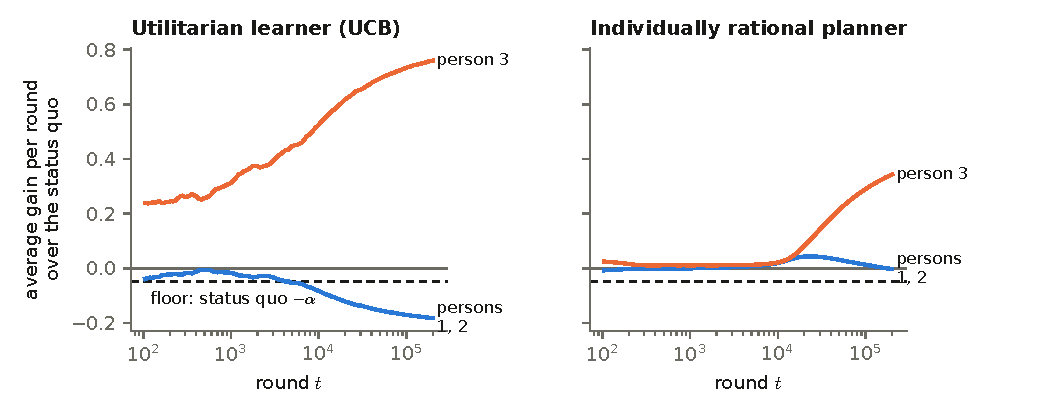
\includegraphics[width=\linewidth]{figures/fig_planner.pdf}
\caption{\Cref{ex:sq}: each person's average gain per round over the status quo, up to round $t$. Left: UCB on the welfare signal finds $\astar$ and takes persons 1 and 2 below the status quo. Right: the individually rational planner of \cref{sec:sq} with $\alpha=0.05$ (mean of 20 runs, band of two standard errors) keeps everyone above the floor and passes most of the gain to person 3.}
\label{fig:planner}
\end{figure}

% ======================================================================
\section{Guarantees or compensation}\label{sec:comp}
% ======================================================================

\Cref{sec:sq} protects each person with a floor of their own. The other way to protect people is to pay them. This section sets up compensation as an institution of the same kind, with its own planner and its own guarantee, so that the two can be compared: on what each aims at, on how fast each can learn, and on what each has to assume.

\subsection{Insure and share}

Suppose rewards are in a common unit that can be moved between people, and that after each round the planner can make transfers $z_t\in\R^N$ with $\sum_iz_{t,i}=0$. Person $i$'s net reward is $X_{t,i}+z_{t,i}$. Write $Y_t=\sum_iX_{t,i}$ for the total.

\begin{definition}[Insure and share]\label{def:insure}
Let $s\ge0$ be shares with $\sum_is_i=1$. The transfers
\[
  z_{t,i}=\big(\mu_{i,a_0}-X_{t,i}\big)+s_i\big(Y_t-W(a_0)\big)
\]
pay each person the difference between their status-quo reward and what they actually received, and then divide the surplus of the round, $Y_t-W(a_0)$, according to the shares. They sum to zero in every round.
\end{definition}

The scheme needs each person's realised reward and status-quo reward. It needs no estimate of anyone's mean under any other policy.

\begin{proposition}[What compensation does]\label{prop:insure}
Under insure-and-share, for every planner and every $T$:
\begin{enumerate}[leftmargin=*,itemsep=1pt,label=(\alph*)]
  \item person $i$'s realised net gain over the status quo is $s_i\sum_{t\le T}(Y_t-W(a_0))$, the same multiple $s_i$ of one number for everyone;
  \item person $i$'s expected shortfall from their share of the best policy, $s_iT(W(\astar)-W(a_0))$, is $s_i\sum_a\Delta_a\E[n_a(T)]$, their share of the collective's regret.
\end{enumerate}
With equal shares and an asymptotically optimal planner every person's burden is $\frac1N\sum_a\Delta_a\cmin_a$ per unit of $\log T$. No consistent planner, with any transfers that sum to zero, has a smaller largest burden.
\end{proposition}

\begin{proof}
(a) $X_{t,i}+z_{t,i}=\mu_{i,a_0}+s_i(Y_t-W(a_0))$; subtract $\mu_{i,a_0}$ and sum over $t$. (b) Take expectations: $\E[Y_t]=\E[W(a_t)]$, and $\sum_t(W(\astar)-W(a_t))=\sum_a\Delta_an_a(T)$. For the last claim, transfers that sum to zero leave the sum of the burdens equal to the collective's regret, so the largest burden is at least a fraction $1/N$ of it, and by \cref{thm:lower} the collective's regret is at least $\sum_a\Delta_a\cmin_a$ per unit of $\log T$ in the limit.
\end{proof}

So compensation removes the per-person problem. Everyone's gain is a fixed share of the same total, including the noise, and everyone therefore wants what the utilitarian planner wants. The largest learning burden falls from $v^\star$ (\cref{sec:fair}) to the lower bound in \cref{prop:lp}: in \cref{ex:blog} from $661$ to $21$ per unit of $\log T$, in \cref{ex:sq} from $691$ to $26$. What remains to be decided is the shares, which is a question of distribution and has nothing to do with learning. Equal shares give each person the same gain. Shares in proportion to each person's gain under $\astar$ among those who gain, and zero for the rest, make the losers whole and leave the winners the remainder.

\subsection{A pooled floor}

Compensation does not remove the need for tolerance. A round in which the planner tries a policy that is worse in total has a negative surplus, and everyone pays a share of it. Under insure-and-share person $i$'s expected net gain in round $t$ is $s_i(W(p_t)-W(a_0))$, so the planner is $\alpha$-individually rational in net terms if and only if
\[
  W(p_t)\ \ge\ W(a_0)-\alpha/\max_is_i ,
\]
which with equal shares is $W(p_t)\ge W(a_0)-N\alpha$. The $N$ floors of \cref{def:ir} have become one floor on welfare, and the $N$ tolerances have been pooled. The planner of \cref{sec:sq} applies with the total in place of a person: a lower confidence bound $\max\{\hat W_a-\sigma r_n,\ W(a_0)-NL\}$ in the constraint, an upper one in the objective, and the same exploring share. It needs only the welfare signal to choose policies. \Cref{prop:nofree,prop:safe,prop:regret} hold with the same proofs; in particular with $\alpha=0$ it still cannot try anything.

Two things change.

\paragraph{The target.} With a floor for each person the planner aims at $p^\star_\alpha$, and gives up $W(\astar)-W_\alpha$ in every round for as long as someone would lose more than $\alpha$ under $\astar$. With a pooled floor it aims at $\astar$, which always satisfies the floor because $W(\astar)\ge W(a_0)$. In \cref{ex:sq} with $\alpha=0.05$ the first settles on welfare $2.97$ with gains $(-0.05,-0.05,+0.47)$ and the second on $3.00$ with gains of $+0.13$ each under equal shares.

\paragraph{The speed.} Before a planner may hold a new policy for a given fraction of the time it has to be confident that doing so respects the floor, and that takes trials. The next proposition bounds the number from below in the simplest case, and compares the two kinds of floor.

\begin{proposition}[Trials needed before a reform can be held]\label{prop:certify}
Let there be two policies, the status quo and a reform $a$, with independent noise. Let $g_i=\mu_{i,a}-\mu_{i,a_0}$ and $G=\sum_ig_i$. Let $q\in(0,1]$ with $\alpha/q<L$, let $\delta<1/2$ and $\kappa_\delta=\tfrac12\log\frac{1}{4\delta(1-\delta)}$. Suppose that on instance $\nu$ there is a round $t$ in which the planner holds the reform at least a fraction $q$ of the time, $p_t(a)\ge q$, with probability at least $1/2$.
\begin{enumerate}[leftmargin=*,itemsep=1pt,label=(\alph*)]
  \item If the planner is $\alpha$-individually rational with confidence $1-\delta$ on $\Env_L$, then $g_i+\alpha/q>0$ for every $i$ and
  \[
    \E_\nu[n_a(t-1)]\ \ge\ \max_i\ \frac{2\sigma_i^2\,\kappa_\delta}{(g_i+\alpha/q)^2}.
  \]
  \item If instead the planner satisfies the pooled floor $W(p_t)\ge W(a_0)-N\alpha$ for all $t$ with probability at least $1-\delta$ on $\Env_L$, and $L$ is large enough for the instance used in the proof to lie in $\Env_L$, then $G+N\alpha/q>0$ and
  \[
    \E_\nu[n_a(t-1)]\ \ge\ \frac{2\sigma^2\,\kappa_\delta}{(G+N\alpha/q)^2}.
  \]
\end{enumerate}
The bound in (b) is never larger than the bound in (a).
\end{proposition}

\begin{proof}
Let $E=\{p_t(a)\ge q\}$, an event determined by the history before round $t$ and the planner's internal randomness. (a) Fix $i$ and $\varepsilon>0$ small, and let $\nu'$ agree with $\nu$ except that $\mu'_{i,a}=\mu_{i,a_0}-\alpha/q-\varepsilon$. On $\nu'$, on $E$, person $i$'s expected reward in round $t$ is $\mu_{i,a_0}-p_t(a)(\alpha/q+\varepsilon)<\mu_{i,a_0}-\alpha$, which violates the floor, so $\Prob_{\nu'}(E)\le\delta$. If $g_i\le-\alpha/q$ the same computation on $\nu$ itself gives $\Prob_\nu(E)\le\delta<1/2$, contrary to the hypothesis; so $g_i+\alpha/q>0$. The two instances differ only in person $i$'s mean under $a$, by $g_i+\alpha/q+\varepsilon$, so by the divergence decomposition and the data-processing inequality,
\[
  \E_\nu[n_a(t-1)]\,\frac{(g_i+\alpha/q+\varepsilon)^2}{2\sigma_i^2}\ \ge\ \mathrm{kl}\big(\Prob_\nu(E),\Prob_{\nu'}(E)\big)\ \ge\ \mathrm{kl}(\tfrac12,\delta)=\kappa_\delta,
\]
where $\mathrm{kl}$ is the divergence between Bernoulli laws, which is increasing in its first argument and decreasing in its second on $\{x>y\}$. Let $\varepsilon\downarrow0$. (b) Let $\nu'$ shift the reform's mean vector by $d$ with $\mathbf 1^\top d=-(G+N\alpha/q+\varepsilon)$, so that on $E$ the welfare of round $t$ is below $W(a_0)-N\alpha$. By \cref{lem:kl} the cheapest such shift costs $(G+N\alpha/q+\varepsilon)^2/(2\sigma^2)$ per trial, and the argument is the same. For the comparison, write $x_i=g_i+\alpha/q>0$. Then $(\sum_ix_i)^2\ge\sum_ix_i^2$, and a ratio of sums is at most the largest ratio of terms, so $\sigma^2/(\sum_ix_i)^2\le\sum_i\sigma_i^2/\sum_ix_i^2\le\max_i\sigma_i^2/x_i^2$.
\end{proof}

With a floor for each person the time is set by the person closest to their floor, and it grows without bound as that person's margin $g_i+\alpha/q$ shrinks. With a pooled floor it is set by the total, where one person's loss is offset by another's gain and the noise is averaged. These are lower bounds for each regime, not rates that our planners attain.

Take \cref{ex:sq} with only the status quo and $\astar$, and $\alpha=\delta=0.05$. Persons 1 and 2 lose $0.2$ under $\astar$, so with per-person floors $\astar$ can never be held more than a quarter of the time. Holding it $20\%$ of the time takes at least $664$ trials; $24\%$ takes at least $23{,}900$. With a pooled floor the corresponding bounds are $4$ and $5$ trials, and adopting $\astar$ outright takes at least $17$.

\subsection{Simulation}

\Cref{fig:compare} runs both planners on \cref{ex:sq}, with all four policies, at $\alpha=0.05$ and $\alpha=0.2$. With $\alpha=0.05$ the pooled planner reaches welfare $2.80$ by $3{,}000$ rounds and $2.96$ by $30{,}000$, and each person is $0.07$ and then $0.12$ per round above the status quo. The planner with per-person floors is at $2.62$ and $2.83$, and its least-favoured person is $0.00$ and $0.04$ above. The pooled planner's welfare never fell more than $0.05$ below the status quo in any round, against a floor of $0.15$.

The figure also shows the utilitarian learner of \cref{sec:score} with compensation and no floor. It does best at every horizon: each person is $0.05$ per round above the status quo at $T=30$ and $0.13$ at $T=30{,}000$. It gives no guarantee for any single round. In a round in which it tries $c$, each person's expected net reward is $0.37$ below the status quo.

\begin{figure}[t]\centering
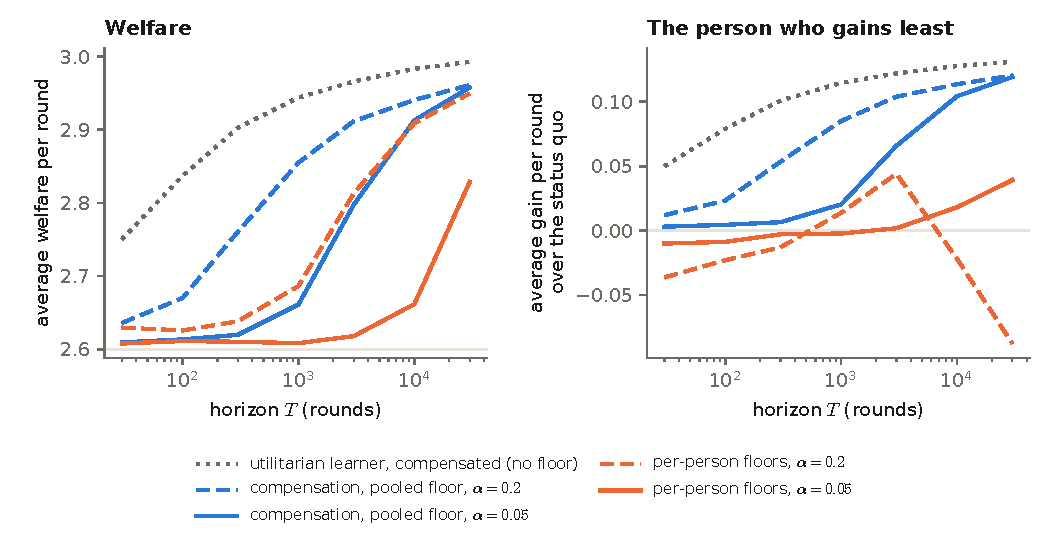
\includegraphics[width=\linewidth]{figures/fig_compare.pdf}
\caption{\Cref{ex:sq}: per-person floors (\cref{sec:sq}) against compensation with a pooled floor and equal shares. Left: welfare per round, averaged over the horizon. Right: the average gain over the status quo of whoever gains least; under compensation everyone gains the same. Means over 40 runs (200 for the utilitarian learner).}
\label{fig:compare}
\end{figure}

\subsection{What each assumes}

Compensation does better on every measure above, and it assumes more.
\begin{itemize}[leftmargin=*,itemsep=1pt]
  \item \emph{A common unit.} Rewards must be transferable one for one. Losses of health, status or liberty are not made good by a payment of equal size, and a person short of money values a payment more than a person who is not.
  \item \emph{Honest, observable outcomes.} The scheme pays each person the gap between their status-quo reward and their realised reward. A person who is fully insured against their own reported outcome has no reason to report it truthfully or to take care over it.
  \item \emph{A known status quo for each person.} The insurance is defined relative to $\mu_{i,a_0}$. Disputes about what someone would have had are disputes about the size of the payment.
  \item \emph{Agreed shares.} The scheme turns a question about policies into a question about dividing a surplus. Equal shares give person 3 in \cref{ex:sq} a gain of $0.13$ where $\astar$ without transfers gives $0.80$.
  \item \emph{Levies.} In a round with a negative surplus the scheme collects from everyone. The floor limits the expected levy, not the realised one.
\end{itemize}
Per-person floors assume none of this. They are what protection costs when people cannot be paid: welfare forgone in every round, and a wait that is set by the person with least to spare.

% ======================================================================
\section{Short horizons and frictions}\label{sec:finite}
% ======================================================================

The results of \cref{sec:lower,sec:exact,sec:cone,sec:fair} describe a regime that \cref{sec:numerics} shows is reached only after about $10^6$ rounds in our own example. A government may get tens of rounds in a policy area. This section says what carries over to short horizons, why the frictions that governments and firms face do not show up in the asymptotic theory, and what a rational planner does in the simplest finite problem.

\paragraph{What carries over.} The identity \eqref{eq:linear}, $\E[R(T)]=D\,\E[n(T)]$, holds for every planner and every $T$. At any horizon, who pays is fixed by which policies are tried and for how long, and a person's cost is their loss under each tried policy times the time it is in force. What does not carry over is the allocation. The asymptotic weights $\cmin_a\propto\Delta_a^{-2}$ come from the requirement of consistency, which says nothing at small $T$. There the natural benchmark is a planner that maximises expected welfare under a prior.

\paragraph{Frictions vanish asymptotically.} A government cannot change policy every round. Changing has a cost, and a policy once adopted stays for a term. In the stochastic bandit neither matters in the limit: with a cost per switch, allocation in growing blocks attains the Lai--Robbins constant with a switching cost of smaller order than $\log T$ \citep{agrawal1988}, and with decisions confined to a small number of batches, of order $\log\log T$, the minimax rate is unchanged \citep{perchet2016,gao2019}. The frictions bite only when the horizon is short, which is one more reason to look there.

\subsection{One status quo, one reform}

The simplest finite problem has a known status quo and a single untried reform. Normalise the status quo's welfare to $0$ per round. The reform's welfare per round is $\theta$, unknown, with prior $\theta\sim\mathcal N(m,1)$, so that welfare is measured in prior standard deviations. While the reform is in force the planner observes $\theta$ plus Gaussian noise of standard deviation $\varsigma$ each round. Policies are held in blocks of $\ell$ rounds (a term), and each change of policy costs $c$. The planner maximises expected total welfare over $T$ rounds, starting from the status quo. We solve the problem numerically by backward induction over the number of rounds the reform has been in force, the posterior mean, and the policy currently in force. We take $\varsigma=3$, so that a single round is weak evidence.

\begin{figure}[t]\centering
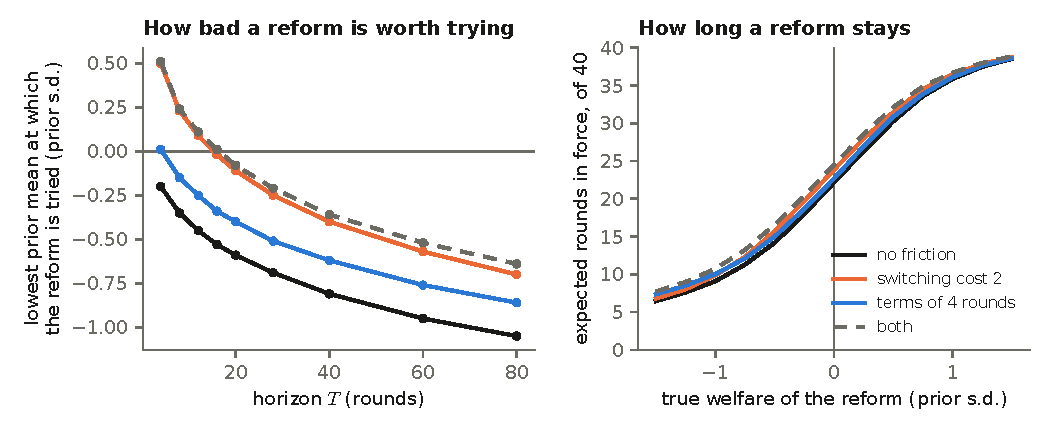
\includegraphics[width=\linewidth]{figures/fig_reform.pdf}
\caption{The one-reform problem with noise $\varsigma=3$. Left: the lowest prior mean $m$ at which the welfare-maximising planner tries the reform. Below zero, the reform is expected to be worse than the status quo. Right: with $T=40$ and $m=0$, the expected number of rounds the reform is in force, as a function of its true welfare (4{,}000 simulated paths per point).}
\label{fig:reform}
\end{figure}

\paragraph{A rational planner tries reforms it expects to be worse.} With no frictions and $T=40$, the planner tries any reform whose prior mean is above $-0.81$ (\cref{fig:reform}, left). It expects such a reform to lose, and tries it because the loss is bounded by the option to stop while the gain, if the reform turns out well, lasts for the rest of the horizon. The threshold falls with the horizon: $-0.20$ at $T=4$, $-0.59$ at $T=20$, $-1.05$ at $T=80$. A planner that tries only reforms it expects to be better than the status quo is leaving welfare unclaimed, and more of it the longer its horizon.

\paragraph{Frictions raise the bar.} A switching cost of $c=2$ moves the threshold at $T=40$ from $-0.81$ to $-0.40$; terms of four rounds move it to $-0.62$. At $T=4$ a term of four rounds removes the option to stop altogether, and the planner tries the reform only if it expects it to be better. With a switching cost the reform must also repay the cost, so the threshold at $T=4$ is $+0.5$. Frictions also keep reforms in force longer once tried, though the effect is small here (\cref{fig:reform}, right): the main effect of commitment and inertia is on which reforms are tried at all.

\paragraph{Bad reforms are tried, and somebody pays.} With $m=0$ and $T=40$, a reform whose true welfare is $-0.5$ stays in force for $14$ rounds on average, and one at $-1$ for $9$. This is the planner working as intended, and the people who lose under that reform bear the cost for those rounds. With a single reform the regret vector lies along one direction: person $i$ loses $\mu_{i,a_0}-\mu_{i,\text{reform}}$ per round for as long as the trial lasts. The per-person question at a short horizon is therefore less about how to split exploration between arms and more about three things the planner controls: which reforms are put on the agenda, how quickly a failing one is stopped, and whether its losers are compensated for the rounds it ran.

With several untried reforms the order in which they are tried decides who pays first, and under a short horizon some will never be tried. We leave that problem open.

% ======================================================================
\section{Comparing institutions}\label{sec:score}
% ======================================================================

Each planner in this paper is a rule for choosing public policies, and so is each of the practices it stands for: keeping what is in force, piloting and then deciding, learning as you go, protecting everyone, taking turns. They can be scored on one card: welfare, each person's gain over the status quo, and the largest conflict loss. We fill in the card for \cref{ex:sq}, first in the long run and then at finite horizons.

\paragraph{The long run.} \Cref{tab:score} gives the policy each institution settles on and what it pays. Every entry is the solution of a linear program.

\begin{table}[h]\centering\small
\begin{tabular}{lcccc}
\toprule
& welfare & \multicolumn{2}{c}{gain over the status quo} & largest\\
institution (long-run policy) & per round & persons 1, 2 & person 3 & conflict loss\\
\midrule
keep the status quo & 2.60 & $0$ & $0$ & 0.80\\
utilitarian learner ($\astar$) & 3.00 & $-0.20$ & $+0.80$ & 0.50\\
utilitarian learner, losers made whole & 3.00 & $0$ & $+0.40$ & --\\
utilitarian learner, surplus shared equally & 3.00 & $+0.13$ & $+0.13$ & --\\
unanimity, $\alpha=0$ ($60\%\ \astar$, $40\%\ b$) & 2.96 & $0$ & $+0.36$ & 0.44\\
tolerance $\alpha=0.05$ ($70\%\ \astar$, $30\%\ b$) & 2.97 & $-0.05$ & $+0.47$ & 0.35\\
smallest largest conflict loss ($69\%\ \astar$, $31\%\ b$) & 2.97 & $-0.04$ & $+0.46$ & 0.34\\
\bottomrule
\end{tabular}
\caption{\Cref{ex:sq}: long-run outcome per round. The two transfer rows are insure-and-share (\cref{def:insure}) with shares $(0,0,1)$ and $(\tfrac13,\tfrac13,\tfrac13)$; they require transferable rewards. The unanimity row is the best outcome that leaves no one worse off; a planner that must also \emph{learn} under $\alpha=0$ never leaves the status quo (\cref{prop:nofree}).}
\label{tab:score}
\end{table}

\paragraph{Finite horizons.} The long-run card leaves out the cost of getting there. For that we run each institution as a planner that starts knowing only the status quo, and record the expected reward it gives each person, averaged over the first $T$ rounds. The planners are:
\begin{itemize}[leftmargin=*,itemsep=1pt]
  \item \emph{keep the status quo}, which is also what a planner bound by unanimity must do;
  \item \emph{adopt $\astar$ at once}, an oracle, for reference;
  \item the \emph{utilitarian learner}: Thompson sampling on the welfare signal, with the status quo's welfare known (UCB behaves similarly and is in the results file);
  \item \emph{pilot, then decide}: try each alternative for $T^{2/3}/(K-1)$ rounds, then keep whichever has the best observed total for the rest of the horizon;
  \item a \emph{time-share} learner, which plays the equal-conflict time-share of \cref{prop:share} computed from current estimates, mixed with uniform exploration of weight $t^{-1/3}$;
  \item the \emph{individually rational} planner of \cref{sec:sq}, with $\alpha=0.05$ and $\alpha=0.2$;
  \item \emph{compensation}: the transfers of \cref{def:insure} with equal shares, on top of the utilitarian learner, and on top of the pooled-floor planner of \cref{sec:comp} with $\alpha=0.05$ and $\alpha=0.2$.
\end{itemize}
The pilot length and the exploration weights are not tuned. \Cref{fig:score,tab:scoreT} report the results.

\begin{figure}[t]\centering
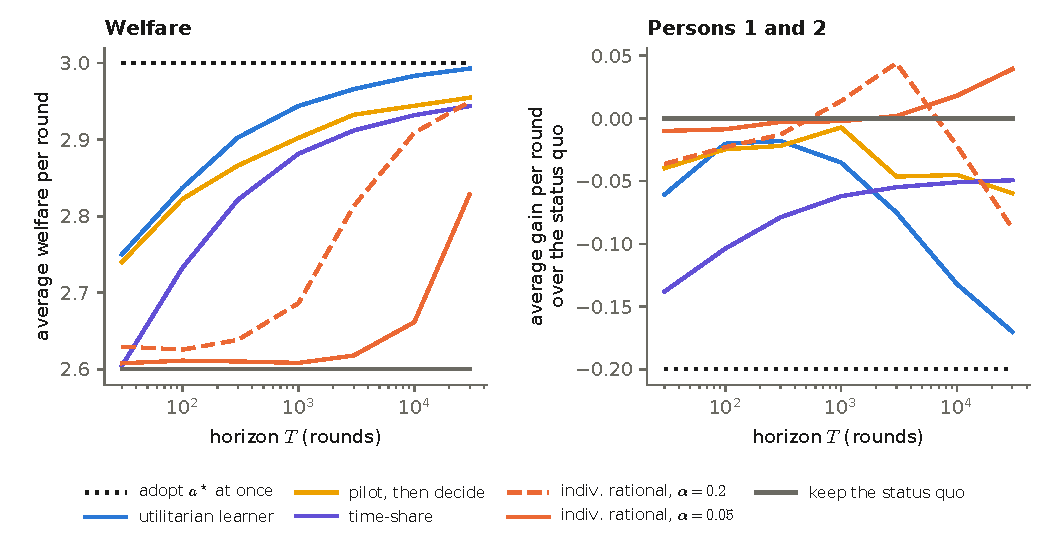
\includegraphics[width=\linewidth]{figures/fig_scorecard.pdf}
\caption{\Cref{ex:sq}: seven institutions without transfers at horizons from $30$ to $30{,}000$ rounds. Left: welfare per round, averaged over the horizon. Right: the average gain of persons 1 and 2, whom the status quo favours. Means over 200 runs (40 for the time-share and individually rational planners).}
\label{fig:score}
\end{figure}

\begin{table}[h]\centering\small
\begin{tabular}{l ccc ccc ccc}
\toprule
& \multicolumn{3}{c}{$T=30$} & \multicolumn{3}{c}{$T=1{,}000$} & \multicolumn{3}{c}{$T=30{,}000$}\\
institution & $W$ & $G_{1,2}$ & $G_3$ & $W$ & $G_{1,2}$ & $G_3$ & $W$ & $G_{1,2}$ & $G_3$\\
\midrule
keep the status quo & 2.60 & $0$ & $0$ & 2.60 & $0$ & $0$ & 2.60 & $0$ & $0$\\
adopt $\astar$ at once & 3.00 & $-.20$ & $+.80$ & 3.00 & $-.20$ & $+.80$ & 3.00 & $-.20$ & $+.80$\\
utilitarian learner & 2.75 & $-.06$ & $+.27$ & 2.94 & $-.04$ & $+.41$ & 2.99 & $-.17$ & $+.73$\\
pilot, then decide & 2.74 & $-.04$ & $+.22$ & 2.90 & $-.01$ & $+.32$ & 2.96 & $-.06$ & $+.47$\\
time-share & 2.61 & $-.14$ & $+.28$ & 2.88 & $-.06$ & $+.41$ & 2.94 & $-.05$ & $+.44$\\
individually rational, $\alpha=0.2$ & 2.63 & $-.04$ & $+.10$ & 2.69 & $+.01$ & $+.06$ & 2.95 & $-.09$ & $+.53$\\
individually rational, $\alpha=0.05$ & 2.61 & $-.01$ & $+.03$ & 2.61 & $-.00$ & $+.01$ & 2.83 & $+.04$ & $+.15$\\
\midrule
utilitarian learner, compensated & 2.75 & $+.05$ & $+.05$ & 2.94 & $+.11$ & $+.11$ & 2.99 & $+.13$ & $+.13$\\
compensation, pooled floor, $\alpha=0.2$ & 2.64 & $+.01$ & $+.01$ & 2.86 & $+.09$ & $+.09$ & 2.96 & $+.12$ & $+.12$\\
compensation, pooled floor, $\alpha=0.05$ & 2.61 & $+.00$ & $+.00$ & 2.66 & $+.02$ & $+.02$ & 2.96 & $+.12$ & $+.12$\\
\bottomrule
\end{tabular}
\caption{\Cref{ex:sq}: welfare per round $W$ and average gain over the status quo for persons 1 and 2 ($G_{1,2}$) and person 3 ($G_3$), averaged over the first $T$ rounds. The last three rows use the transfers of \cref{def:insure} with equal shares. Standard errors of $W$ are at most $0.02$ at $T=30$ and $0.01$ at the longer horizons.}
\label{tab:scoreT}
\end{table}

Four things stand out.

\emph{Learning at all matters more than how.} At $T=30$ the utilitarian learner and the pilot both reach about $2.75$, against $2.60$ for the status quo and $3.00$ for the oracle. The gap between them is small next to the gap between either and doing nothing.

\emph{The cost to the people the status quo favours arrives late.} Under the utilitarian learner, persons 1 and 2 lose $0.02$ to $0.06$ per round at horizons up to $1{,}000$, and $0.17$ at $30{,}000$. Early on the learner spends much of its time on $b$, which they prefer; as it becomes sure of $\astar$ it stops. At short horizons a utilitarian learner behaves like a time-share without intending to.

\emph{Compensation is affordable at every horizon.} Holding persons 1 and 2 at their status-quo level under the utilitarian learner would take transfers of between $0.04$ and $0.34$ per round, depending on the horizon. That is between $12\%$ and $87\%$ of the welfare the learner gains over the status quo, and never more than it. With the surplus shared equally, everyone is above the status quo in expectation at each of the horizons we ran.

\emph{A guarantee is expensive in time, tolerance buys speed, and pooling buys more.} With $\alpha=0.05$ the individually rational planner gains almost nothing for $10^4$ rounds; by $30{,}000$ it has everyone above the status quo, at welfare $2.83$. With $\alpha=0.2$ it has everyone above the status quo by $3{,}000$ rounds. With compensation and a pooled floor at $\alpha=0.05$, welfare is $2.96$ at $30{,}000$ rounds and everyone gains from the first round (\cref{sec:comp}). A collective that insists on a tight per-person guarantee without transfers and has a short horizon gets, in effect, the status quo.

These are expectations on one example with three people, and the ranking will change with the instance. What the exercise shows is that the institutions can be compared on common terms, and that the comparison depends strongly on the horizon.


% ======================================================================
\section{Numerical illustrations for the asymptotic results}\label{sec:numerics}
% ======================================================================

All numbers in this section are produced by \texttt{code/scripts/simulate.py}, and those in \cref{sec:sharing,sec:sq,sec:finite} by \texttt{code/scripts/extensions.py} and those in \cref{sec:score} by \texttt{code/scripts/scorecard.py}; the tests in \texttt{code/tests/} compare simulations and independent computations with the closed forms above. Planners observe only the welfare signal.

\paragraph{Convergence is slow.} The theorems are statements about $T\to\infty$, and for small gaps the approach is slow. \Cref{tab:conv} reports $\E[R_i(T)]/\log T$ for \cref{ex:blog} over 20 seeds. For UCB, the count of the near-tie arm $b$ (gap-to-noise ratio $\Delta_b/\sigma\approx0.06$) reaches its asymptotic rate only at $T\approx10^6$; for the large-gap arm $c$, UCB stays about $30\%$ above the limit, consistent with the $2\log\log T$ term in $\log f(T)$. Thompson sampling is far below the limit at every horizon we ran, at about $40\%$ of the asymptotic count for $b$ at $T=10^6$; this is not a contradiction, since \cref{thm:lower} is asymptotic and its finite-$T$ form subtracts a term that is large for near-ties. The per-person \emph{ratios} are nevertheless as predicted at every horizon, because both planners spend almost all their exploration on $b$: the ratio of person 3's burden to person 1's gain is $2.21$ in the limit and between $2.2$ and $2.4$ in every simulated row (\cref{fig:traj}).

\begin{table}[h]\centering\small
\begin{tabular}{rrrrr|rrrr}
\toprule
& \multicolumn{4}{c|}{UCB on the welfare signal} & \multicolumn{4}{c}{Thompson sampling}\\
$T$ & $R_1/\log T$ & $R_3/\log T$ & $\frac{n_b}{\cmin_b\log T}$ & $\frac{n_c}{\cmin_c\log T}$ & $R_1/\log T$ & $R_3/\log T$ & $\frac{n_b}{\cmin_b\log T}$ & $\frac{n_c}{\cmin_c\log T}$\\
\midrule
$10^3$ & $-24.1$ & $57.1$ & 0.08 & 0.95 & $-26.5$ & $60.7$ & 0.09 & 0.54\\
$10^4$ & $-95.8$ & $216.2$ & 0.32 & 1.27 & $-93.9$ & $209.2$ & 0.32 & 0.60\\
$10^5$ & $-203.1$ & $452.6$ & 0.68 & 1.32 & $-107.5$ & $239.3$ & 0.36 & 0.66\\
$10^6$ & $-302.4$ & $670.9$ & 1.01 & 1.34 & $-122.6$ & $272.5$ & 0.41 & 0.65\\
\midrule
limit & $-298.7$ & $661.3$ & 1 & 1 & $-298.7$ & $661.3$ & 1 & 1\\
\bottomrule
\end{tabular}
\caption{\Cref{ex:blog}: mean over 20 seeds of per-person regret per unit of $\log T$ (person 2 equals person 1), and counts relative to the Lai--Robbins rate. Standard errors at $T=10^6$: $20$ and $45$ (UCB), $15$ and $33$ (Thompson sampling) for $R_1$ and $R_3$.}
\label{tab:conv}
\end{table}

\begin{figure}[h]\centering
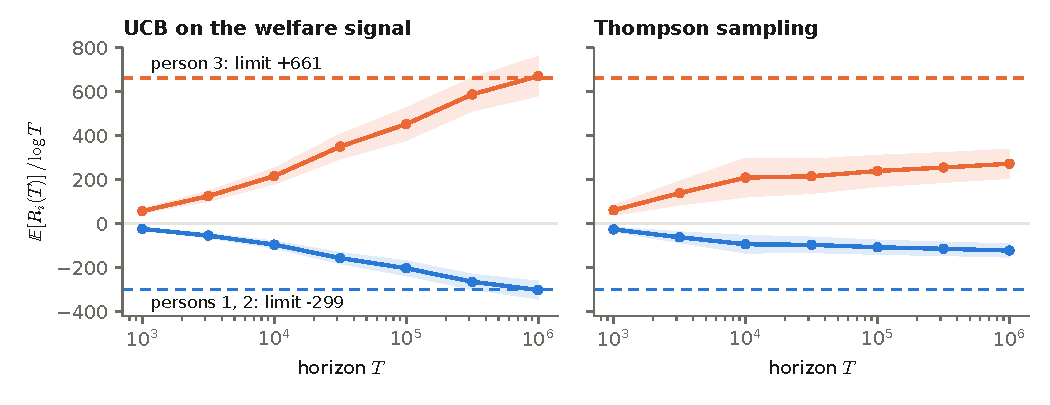
\includegraphics[width=\linewidth]{figures/fig_trajectories.pdf}
\caption{\Cref{ex:blog}: simulated $\E[R_i(T)]/\log T$ (mean over 20 seeds, band of two standard errors) against the limits of \cref{thm:exact} (dashed). UCB reaches the limit near $T=10^6$; Thompson sampling is still well short of it.}
\label{fig:traj}
\end{figure}

\paragraph{The cone at finite $T$.} The forced-exploration construction of \cref{thm:cone} shifts the burden vector by exactly $Dg\log T$ relative to the base planner, plus lower-order terms, \emph{whether or not the base planner has converged}, because the base planner runs on its own samples. In \cref{ex:comp}, with the min-max rates $g_d=810$, the predicted shift is $Dg=(324,324,-486)$ per unit of $\log T$; the observed shifts are reported in \cref{tab:shift}; at $T=10^6$ they are within about one standard error of the prediction for both base planners. Reaching the min-max point itself at finite $T$ is limited by the base planner's convergence, not by the construction.

\begin{table}[h]\centering\small
\begin{tabular}{rrr|rr}
\toprule
& \multicolumn{2}{c|}{UCB base} & \multicolumn{2}{c}{Thompson base}\\
$T$ & persons 1, 2 & person 3 & persons 1, 2 & person 3\\
\midrule
$10^4$ & 373.9 & $-611.2$ & 354.6 & $-556.8$\\
$10^5$ & 363.7 & $-576.4$ & 316.9 & $-468.1$\\
$10^6$ & 354.4 & $-553.0$ & 312.8 & $-459.8$\\
\midrule
predicted $Dg$ & 324.0 & $-486.0$ & 324.0 & $-486.0$\\
\bottomrule
\end{tabular}
\caption{\Cref{ex:comp}: difference in mean per-person regret per unit of $\log T$ between the forced-exploration planner ($g_d=810$) and its base planner, from two independent sets of 20 seeds. Standard errors of the difference at $T=10^6$ are roughly $35$ (persons 1, 2) and $80$ (person 3). At $T=10^4$ the forced pulls ($\approx 7{,}500$) take most of the rounds, so the base planner has had only $S(T)\approx2{,}500$ steps; this inflates the observed shift at small $T$.}
\label{tab:shift}
\end{table}

\paragraph{How often is the utilitarian planner unimprovable?} We drew 400 instances for each of four sizes, with $\mu_{i,a}$ i.i.d.\ standard normal, independent noise and $\sigma_i$ uniform on $[0.5,1.5]$, and solved the min-max LP. \Cref{tab:freq} reports the fraction of instances in which the utilitarian planner is already min-max optimal (certified by \cref{prop:ville} and confirmed by the LP), and, for the remaining instances, the median relative reduction in the worst burden and the median relative increase in total regret. Under this instance distribution the utilitarian planner is unimprovable in most instances; where it is not, small reductions in the worst burden cost large increases in total regret. These frequencies depend on the instance distribution and should be read as illustrations, not as estimates for any real population.

\begin{table}[h]\centering\small
\begin{tabular}{rrccc}
\toprule
$N$ & $K$ & unimprovable & median reduction in worst burden & median increase in total regret\\
\midrule
3 & 3 & 93\% & 8.1\% & 49\%\\
5 & 4 & 90\% & 4.1\% & 73\%\\
10 & 5 & 90\% & 3.4\% & 67\%\\
20 & 8 & 79\% & 1.8\% & 52\%\\
\bottomrule
\end{tabular}
\caption{400 random instances per row ($\mu_{i,a}\sim\mathcal N(0,1)$ i.i.d., $\sigma_i\sim U[0.5,1.5]$). ``Unimprovable'': the utilitarian planner is min-max optimal. The medians are over the remaining instances and are relative to the utilitarian planner's worst burden and total regret.}
\label{tab:freq}
\end{table}

% ======================================================================
\section{Related work}\label{sec:related}
% ======================================================================

\paragraph{Lower bounds.} \Cref{thm:lower} is an instance of the classical change-of-measure lower bound \citep{lai1985} in the form presented by \citet{lattimore2020} and \citet{garivier2019}; its only specific content is the minimisation in \cref{lem:kl}. Structured classes are covered by \citet{graves1997} and \citet{combes2017}. Asymptotically optimal algorithms for Gaussian rewards include KL-UCB \citep{cappe2013}, the UCB variant of \citet[Ch.~8]{lattimore2020}, and Thompson sampling \citep{korda2013}.

\paragraph{The same model with a scalar regret.} \citet{hossain2021} introduce the model we use: one arm is applied to all agents, who have different mean rewards for it. Their target is the distribution over arms that maximises Nash social welfare, and they bound a scalar regret against it; \citet{jones2023} improve the rate. \citet{barman2023} study Nash regret, aggregating over rounds. These papers settle what to aim at and collapse the cost of getting there to one number. We keep the vector, first for the utilitarian target and then, in \cref{sec:sharing,sec:sq}, for time-shares of their kind, where the per-person learning cost is open.

\paragraph{Who bears exploration.} The closest work in spirit is \citet{baek2021,baek2024}. In their grouped bandit each round belongs to one group, which pulls an arm from its own set; arm means are shared, so one group's exploration informs the others. They describe the set of per-group gains achievable by consistent policies, show that regret-optimal policies can be arbitrarily unfair, and give a policy that attains the Nash bargaining solution with a bounded price of fairness. Our achievable cone and min-max point are the counterparts of their set and their fair point. The mechanism differs: their burden arises from who pulls an arm, ours from different losses under a common pull, where some people gain; and with a public arm the lever they use is absent. \citet{blanchard2025} minimise the largest regret across groups in a grouped model, non-asymptotically, which is the objective of \cref{sec:fair} in a different setting. \citet{jung2020} show that an agent who can observe a self-reliant learner gets bounded regret while the learner's grows logarithmically, and \citet{wang2023} show that heterogeneous agents can explore for each other for free; both are cases of the sign pattern in $D$, with separate pulls. A planner that reaches a chosen point of our cone on every instance, as PF-UCB does for the bargaining solution, would track the solution of the linear program at the estimated instance, as OSSB does for the Graves--Lai program \citep{combes2017,degenne2020}.

\paragraph{Other fairness notions in bandits.} The fairness notion of \citet{joseph2016} concerns how arms (individuals being selected) are treated, not who bears exploration. Multi-objective bandits with Pareto regret \citep{drugan2013} have vector rewards but a single decision maker and a scalar regret relative to the Pareto front.

\paragraph{Baselines and safety.} Conservative bandits \citep{wu2016} keep cumulative reward above a fraction of a baseline policy's; stage-wise and safe linear bandits impose a constraint in every round \citep{moradipari2020,amani2019}. The planner of \cref{sec:sq} uses the same optimism and pessimism with one constraint per person on a shared arm, which we have not found treated.

\paragraph{Collective experimentation in economics.} \citet{strulovici2010} is the closest economic precursor: voters with different, initially unknown payoffs from a public risky policy decide by vote whether to keep trying it, and experiment too little, because each fears being a loser who can no longer stop the experiment. \citet{fernandez1991} show that uncertainty about who will win can block a reform that a majority would approve after the fact. \citet{anesi2021} show that transfers restore efficient experimentation where veto rights do not. Those models have strategic voters and no planner; ours has a planner and no strategic behaviour, and asks what the planner's learning costs each person.

\paragraph{Externalities of exploration and incentives.} \citet{raghavan2018} study how exploration imposes costs on the users who arrive while it happens. Incentivised exploration \citep{kremer2014,mansour2020} asks how a planner can induce self-interested arrivals to explore; there the explorers could refuse. Strategic experimentation \citep{bolton1999,keller2005} studies agents who each bear their own exploration cost while information is public. Our people cannot refuse; adding exit or voice to the per-person accounting is open.

\paragraph{Frictions.} Switching costs leave the Lai--Robbins constant unchanged \citep{agrawal1988}, and a small number of batches leaves the minimax rate unchanged \citep{perchet2016,gao2019}; see \cref{sec:finite}.

\paragraph{Experimenting on people.} \citet{bird2016} raise the question of who bears the cost when deployed systems experiment on their users. \citet{meyer2015} argues that rolling out an untested policy to everyone is itself an experiment without a control, and \citet{meyer2019} find that people object to a randomised comparison of two policies that they would accept if either were simply imposed. Clinical research has the most developed norms, built on equipoise, stopping rules and consent \citep{freedman1987}.

\paragraph{Distortion.} In social choice, distortion is the welfare lost because a rule sees only part of people's preferences \citep{procaccia2006}; a few cardinal queries reduce it sharply \citep{amanatidis2021}. In \cite{telfar2026} the same quantity measures what a ballot loses by deciding coupled issues separately. It is the middle term of the three in \cref{sec:intro}, and we do not treat it here.

% ======================================================================
\section{Discussion}\label{sec:discussion}
% ======================================================================

\paragraph{Who pays for learning.} Under utilitarian learning of a public policy, the cost concentrates on people who lose from policies that are nearly as good as the best in total and contested. Those are the policies that have to be tried most, and their losers pay a share far above $1/N$. People who prefer such a policy gain while it is tested. The people whose burden nothing can reduce are those for whom the eventual policy is the best there is.

\paragraph{What the planner can do.} A planner committed to $\astar$ can only try some arms more often (\cref{thm:cone}), which helps a person only through an arm that person prefers to $\astar$ and always raises total regret; in most random instances it cannot lower the largest burden at all (\cref{prop:ville}). A planner willing to hold policies in rotation can do much more (\cref{sec:sharing}), at a welfare price that is smallest for exactly the near-ties that are most expensive to resolve. A planner that must leave nobody worse off than the status quo cannot begin without some tolerance (\cref{prop:nofree}), and with it can be made safe by construction (\cref{prop:safe}). A planner that can pay people has the easiest task: the per-person problem reduces to the scalar one, with one floor in place of $N$ (\cref{sec:comp}).

\paragraph{What this suggests for governments and firms.} The following are suggestions that the results support, not conclusions that they prove; each is tied to the result behind it.
\begin{enumerate}[leftmargin=*,itemsep=2pt]
  \item \emph{Keep the per-person account.} The total hides transfers between people that can be ten times its size (\cref{ex:blog}), and it cannot be reconstructed from aggregate outcomes (\cref{rem:noinfo}). Who is exposed, what it costs them and when it ends have to be measured.
  \item \emph{Treat the status quo as a policy.} Keeping it has a regret vector, which falls on the people it serves worst (\cref{sec:sq}).
  \item \emph{Where people can be paid, compensate; keep floors for what cannot be paid for.} Compensation equalises the cost of learning, aims at the best policy and learns faster (\cref{sec:comp}); in our example everyone gains at every horizon. It assumes transferable rewards and honest reporting. Where those fail, per-person floors are the fallback, and their cost in welfare and time should be expected (\cref{prop:certify}). A veto with no tolerance blocks everything (\cref{prop:nofree,tab:ir}).
  \item \emph{Share near-ties.} Where two policies are close in total and far apart in who they serve, resolving the tie costs the most and matters the least for welfare (\cref{sec:sharing}). Rotation, regional variation or opt-outs give each side part of what it wants.
  \item \emph{State the tolerance.} No experiment on a public policy is free of expected loss for everyone (\cref{prop:nofree}). Choosing $\alpha$ openly is better than choosing it by default.
  \item \emph{Try reforms that are expected to be slightly worse, where stopping is cheap.} The option to stop is worth more the longer the horizon and the lower the cost of reversal (\cref{sec:finite}). Long terms and costly reversals are reasons to try less, and to make policies easier to reverse.
  \item \emph{Make the arm private where possible.} Staged rollouts, pilots and sandboxes choose who is exposed, which a public arm does not allow. Our results describe what is lost when that choice is unavailable.
\end{enumerate}
A firm differs from a government in one respect that matters here: its customers can leave. Exit caps what any one person can be made to bear, and it changes the population the firm learns from; we have not modelled it.

\paragraph{AI deployment.} A model release, a change to a recommender, or a regulatory regime for AI systems is close to a public arm for the population it applies to. Staged rollouts, limited releases and regulatory sandboxes are ways of privatising the arm. The results above say that this choice is where most of the leverage over the distribution of the cost of learning lies, and that the previous version of a system is a status quo in the sense of \cref{sec:sq}: users who were well served by it are the privileged of \cref{def:privilege}, and an update is a reform.

% ======================================================================
\section{Limitations and future work}\label{sec:limits}
% ======================================================================

\begin{itemize}[leftmargin=*,itemsep=2pt]
  \item \textbf{Asymptotics.} The results of \cref{sec:lower,sec:exact,sec:cone,sec:fair} are about the $\log T$ rate, and \cref{sec:numerics} shows that convergence is slow for near-ties. \Cref{sec:finite} treats a short horizon only for a single reform. The problem with several untried reforms, where the order of trials decides who pays, is open.
  \item \textbf{Loose bounds for the new planners.} The $T^{2/3}$ bound of \cref{prop:regret} has unoptimised constants and is probably not the right rate; the lower bounds of \cref{prop:certify} are for two policies and are not matched. Compensation is analysed without strategic reporting, which is where it is most exposed. The per-person cost of learning a time-share is not characterised. A planner that reaches the min-max point of the cone on every instance without knowing it has not been constructed.
  \item \textbf{Expectations.} We describe $\E[R(T)]$. The realised regret vector has a distribution, and its tails may matter more to the people concerned.
  \item \textbf{Model.} Gaussian rewards with known covariance, stationary means, an unstructured class and a unique optimum. Other exponential families change the constants through the KL divergence; structured classes change them more substantially (\cref{rem:noinfo}).
  \item \textbf{Known status quo and a known bound.} \Cref{sec:sq} assumes the status-quo means are known exactly and that a bound $L$ on the loss from any policy is known. The tolerance $\alpha$ is in expectation per round; realised losses can be larger.
  \item \textbf{No strategic behaviour.} People report honestly and cannot exit, organise or refuse. All of these would change what the planner observes.
  \item \textbf{One example.} The scorecard of \cref{sec:score} is for a single instance with three people, with planners that are not tuned.
  \item \textbf{Random instances.} The frequencies in \cref{tab:freq,tab:share,tab:ir} depend on the chosen instance distribution, in which people's rewards are independent. Populations with shared interests would look different.
  \item \textbf{Voting and ballots.} The planner here observes rewards. An institution that observes votes converges to something other than $\astar$, and the gap is the distortion term of \cref{sec:intro}. Closing the loop, with a ballot as the feedback channel and the per-person accounts of this paper as the outcome, would combine this paper with \cite{telfar2026}; so would taking policies to be bundles of issue decisions, a structured class in the sense of \cref{rem:noinfo}.
\end{itemize}

\bibliographystyle{plainnat}
\bibliography{references}

\end{document}
